% -*- latex -*-
%----------------------------------------------------------------------------
%
%  Title       :  An Algebra of Sequential Decision Problems
%  Conference: :  MPC 2019
%  Author(s)   :  Robert Krook, Patrik Jansson
%  Copyright   :  TBD
%  Created     :  2019-04-12
%
%  Purpose : Build up a library of combinators for creating SeqDecProbs.
%            In the process, understand the design space better.
%
%----------------------------------------------------------------------------

% \documentclass[sigplan,review,anonymous]{acmart}\settopmatter{printfolios=true,printccs=false,printacmref=false}
\documentclass[sigplan,review]{acmart}\settopmatter{printfolios=true,printccs=false,printacmref=false}

%% Conference information
%% Supplied to authors by publisher for camera-ready submission;
%% use defaults for review submission.
\acmConference[TyDe'19]{ACM SIGPLAN TODO}{August 18, 2019}{Berlin, Germany}
\acmYear{2019}
\acmISBN{} % \acmISBN{978-x-xxxx-xxxx-x/YY/MM}
\acmDOI{} % \acmDOI{10.1145/nnnnnnn.nnnnnnn}
\startPage{1}

\setcopyright{none} %**TODO
\bibliographystyle{ACM-Reference-Format}

%%% Standard definitions from the lhs2TeX installation
%% ODER: format ==         = "\mathrel{==}"
%% ODER: format /=         = "\neq "
%
%
\makeatletter
\@ifundefined{lhs2tex.lhs2tex.sty.read}%
  {\@namedef{lhs2tex.lhs2tex.sty.read}{}%
   \newcommand\SkipToFmtEnd{}%
   \newcommand\EndFmtInput{}%
   \long\def\SkipToFmtEnd#1\EndFmtInput{}%
  }\SkipToFmtEnd

\newcommand\ReadOnlyOnce[1]{\@ifundefined{#1}{\@namedef{#1}{}}\SkipToFmtEnd}
\usepackage{amstext}
\usepackage{amssymb}
\usepackage{stmaryrd}
\DeclareFontFamily{OT1}{cmtex}{}
\DeclareFontShape{OT1}{cmtex}{m}{n}
  {<5><6><7><8>cmtex8
   <9>cmtex9
   <10><10.95><12><14.4><17.28><20.74><24.88>cmtex10}{}
\DeclareFontShape{OT1}{cmtex}{m}{it}
  {<-> ssub * cmtt/m/it}{}
\newcommand{\texfamily}{\fontfamily{cmtex}\selectfont}
\DeclareFontShape{OT1}{cmtt}{bx}{n}
  {<5><6><7><8>cmtt8
   <9>cmbtt9
   <10><10.95><12><14.4><17.28><20.74><24.88>cmbtt10}{}
\DeclareFontShape{OT1}{cmtex}{bx}{n}
  {<-> ssub * cmtt/bx/n}{}
\newcommand{\tex}[1]{\text{\texfamily#1}}	% NEU

\newcommand{\Sp}{\hskip.33334em\relax}


\newcommand{\Conid}[1]{\mathit{#1}}
\newcommand{\Varid}[1]{\mathit{#1}}
\newcommand{\anonymous}{\kern0.06em \vbox{\hrule\@width.5em}}
\newcommand{\plus}{\mathbin{+\!\!\!+}}
\newcommand{\bind}{\mathbin{>\!\!\!>\mkern-6.7mu=}}
\newcommand{\rbind}{\mathbin{=\mkern-6.7mu<\!\!\!<}}% suggested by Neil Mitchell
\newcommand{\sequ}{\mathbin{>\!\!\!>}}
\renewcommand{\leq}{\leqslant}
\renewcommand{\geq}{\geqslant}
\usepackage{polytable}

%mathindent has to be defined
\@ifundefined{mathindent}%
  {\newdimen\mathindent\mathindent\leftmargini}%
  {}%

\def\resethooks{%
  \global\let\SaveRestoreHook\empty
  \global\let\ColumnHook\empty}
\newcommand*{\savecolumns}[1][default]%
  {\g@addto@macro\SaveRestoreHook{\savecolumns[#1]}}
\newcommand*{\restorecolumns}[1][default]%
  {\g@addto@macro\SaveRestoreHook{\restorecolumns[#1]}}
\newcommand*{\aligncolumn}[2]%
  {\g@addto@macro\ColumnHook{\column{#1}{#2}}}

\resethooks

\newcommand{\onelinecommentchars}{\quad-{}- }
\newcommand{\commentbeginchars}{\enskip\{-}
\newcommand{\commentendchars}{-\}\enskip}

\newcommand{\visiblecomments}{%
  \let\onelinecomment=\onelinecommentchars
  \let\commentbegin=\commentbeginchars
  \let\commentend=\commentendchars}

\newcommand{\invisiblecomments}{%
  \let\onelinecomment=\empty
  \let\commentbegin=\empty
  \let\commentend=\empty}

\visiblecomments

\newlength{\blanklineskip}
\setlength{\blanklineskip}{0.66084ex}

\newcommand{\hsindent}[1]{\quad}% default is fixed indentation
\let\hspre\empty
\let\hspost\empty
\newcommand{\NB}{\textbf{NB}}
\newcommand{\Todo}[1]{$\langle$\textbf{To do:}~#1$\rangle$}

\EndFmtInput
\makeatother
%
%
%
%
%
%
% This package provides two environments suitable to take the place
% of hscode, called "plainhscode" and "arrayhscode". 
%
% The plain environment surrounds each code block by vertical space,
% and it uses \abovedisplayskip and \belowdisplayskip to get spacing
% similar to formulas. Note that if these dimensions are changed,
% the spacing around displayed math formulas changes as well.
% All code is indented using \leftskip.
%
% Changed 19.08.2004 to reflect changes in colorcode. Should work with
% CodeGroup.sty.
%
\ReadOnlyOnce{polycode.fmt}%
\makeatletter

\newcommand{\hsnewpar}[1]%
  {{\parskip=0pt\parindent=0pt\par\vskip #1\noindent}}

% can be used, for instance, to redefine the code size, by setting the
% command to \small or something alike
\newcommand{\hscodestyle}{}

% The command \sethscode can be used to switch the code formatting
% behaviour by mapping the hscode environment in the subst directive
% to a new LaTeX environment.

\newcommand{\sethscode}[1]%
  {\expandafter\let\expandafter\hscode\csname #1\endcsname
   \expandafter\let\expandafter\endhscode\csname end#1\endcsname}

% "compatibility" mode restores the non-polycode.fmt layout.

\newenvironment{compathscode}%
  {\par\noindent
   \advance\leftskip\mathindent
   \hscodestyle
   \let\\=\@normalcr
   \let\hspre\(\let\hspost\)%
   \pboxed}%
  {\endpboxed\)%
   \par\noindent
   \ignorespacesafterend}

\newcommand{\compaths}{\sethscode{compathscode}}

% "plain" mode is the proposed default.
% It should now work with \centering.
% This required some changes. The old version
% is still available for reference as oldplainhscode.

\newenvironment{plainhscode}%
  {\hsnewpar\abovedisplayskip
   \advance\leftskip\mathindent
   \hscodestyle
   \let\hspre\(\let\hspost\)%
   \pboxed}%
  {\endpboxed%
   \hsnewpar\belowdisplayskip
   \ignorespacesafterend}

\newenvironment{oldplainhscode}%
  {\hsnewpar\abovedisplayskip
   \advance\leftskip\mathindent
   \hscodestyle
   \let\\=\@normalcr
   \(\pboxed}%
  {\endpboxed\)%
   \hsnewpar\belowdisplayskip
   \ignorespacesafterend}

% Here, we make plainhscode the default environment.

\newcommand{\plainhs}{\sethscode{plainhscode}}
\newcommand{\oldplainhs}{\sethscode{oldplainhscode}}
\plainhs

% The arrayhscode is like plain, but makes use of polytable's
% parray environment which disallows page breaks in code blocks.

\newenvironment{arrayhscode}%
  {\hsnewpar\abovedisplayskip
   \advance\leftskip\mathindent
   \hscodestyle
   \let\\=\@normalcr
   \(\parray}%
  {\endparray\)%
   \hsnewpar\belowdisplayskip
   \ignorespacesafterend}

\newcommand{\arrayhs}{\sethscode{arrayhscode}}

% The mathhscode environment also makes use of polytable's parray 
% environment. It is supposed to be used only inside math mode 
% (I used it to typeset the type rules in my thesis).

\newenvironment{mathhscode}%
  {\parray}{\endparray}

\newcommand{\mathhs}{\sethscode{mathhscode}}

% texths is similar to mathhs, but works in text mode.

\newenvironment{texthscode}%
  {\(\parray}{\endparray\)}

\newcommand{\texths}{\sethscode{texthscode}}

% The framed environment places code in a framed box.

\def\codeframewidth{\arrayrulewidth}
\RequirePackage{calc}

\newenvironment{framedhscode}%
  {\parskip=\abovedisplayskip\par\noindent
   \hscodestyle
   \arrayrulewidth=\codeframewidth
   \tabular{@{}|p{\linewidth-2\arraycolsep-2\arrayrulewidth-2pt}|@{}}%
   \hline\framedhslinecorrect\\{-1.5ex}%
   \let\endoflinesave=\\
   \let\\=\@normalcr
   \(\pboxed}%
  {\endpboxed\)%
   \framedhslinecorrect\endoflinesave{.5ex}\hline
   \endtabular
   \parskip=\belowdisplayskip\par\noindent
   \ignorespacesafterend}

\newcommand{\framedhslinecorrect}[2]%
  {#1[#2]}

\newcommand{\framedhs}{\sethscode{framedhscode}}

% The inlinehscode environment is an experimental environment
% that can be used to typeset displayed code inline.

\newenvironment{inlinehscode}%
  {\(\def\column##1##2{}%
   \let\>\undefined\let\<\undefined\let\\\undefined
   \newcommand\>[1][]{}\newcommand\<[1][]{}\newcommand\\[1][]{}%
   \def\fromto##1##2##3{##3}%
   \def\nextline{}}{\) }%

\newcommand{\inlinehs}{\sethscode{inlinehscode}}

% The joincode environment is a separate environment that
% can be used to surround and thereby connect multiple code
% blocks.

\newenvironment{joincode}%
  {\let\orighscode=\hscode
   \let\origendhscode=\endhscode
   \def\endhscode{\def\hscode{\endgroup\def\@currenvir{hscode}\\}\begingroup}
   %\let\SaveRestoreHook=\empty
   %\let\ColumnHook=\empty
   %\let\resethooks=\empty
   \orighscode\def\hscode{\endgroup\def\@currenvir{hscode}}}%
  {\origendhscode
   \global\let\hscode=\orighscode
   \global\let\endhscode=\origendhscode}%

\makeatother
\EndFmtInput
%
%%% Put your own formatting directives in a separate file
% %format (getstate x) = "\getstate{" x "}"


\newcommand{\un}{\mbox{\texttt{\_}}}   % short underscore
\newcommand{\unopun}[1]{\ensuremath{\,\un{#1}\un\,}}

















\usepackage{graphicx}
\usepackage{booktabs}   %% For formal tables:
                        %% http://ctan.org/pkg/booktabs
\usepackage{subcaption}
\usepackage{hyperref}
% \usepackage{color}
\renewcommand\UrlFont{\color{blue}\rmfamily}
\usepackage{doi}

%for agda
\RequirePackage[T1]{fontenc}
\RequirePackage[utf8x]{inputenc}
\RequirePackage{ucs}

% macro for monus operator (credit: https://tex.stackexchange.com/questions/147788/monus-operator-macro)
\providecommand{\dotdiv}{% Don't redefine it if available
  \mathbin{% We want a binary operation
    \vphantom{+}% The same height as a plus or minus
    \text{% Change size in sub/superscripts
      \mathsurround=0pt % To be on the safe side
      \ooalign{% Superimpose the two symbols
        \noalign{\kern-.35ex}% but the dot is raised a bit
        \hidewidth$\smash{\cdot}$\hidewidth\cr % Dot
        \noalign{\kern.35ex}% Backup for vertical alignment
        $-$\cr % Minus
      }%
    }%
  }%
}

%manually added unicode characters
\DeclareUnicodeCharacter{8759}{::}
\DeclareUnicodeCharacter{8760}{\dotdiv}
\DeclareUnicodeCharacter{8644}{\rightleftarrows}
\DeclareUnicodeCharacter{7511}{^{t}}

\usepackage{amssymb}
\usepackage{bbm}
\usepackage[greek,english]{babel}
\usepackage{autofe}
\usepackage{agda}

%%% Some useful macros
\newcommand{\todo}[2][?]{\marginpar{\raggedright \tiny TODO: #2}}
\newcommand{\TODO}[1]{\todo{#1}}
\newcommand{\refSec}[1]{Sec. \ref{#1}}
\newcommand{\refSecs}[1]{Secs. \ref{#1}}
\newcommand{\refSecI}[1]{Section \ref{#1}}
\newcommand{\refSecsI}[1]{Sections \ref{#1}}
\newcommand{\refTab}[1]{Tab. \ref{#1}}

% \newcommand{\getstate}[1]{\ensuremath{\left||#1\right||}}
\newcommand{\getstate}[1]{\ensuremath{\##1}}
%\mathchardef\mhyphen="2D

% -------------------------------------------------------------------------------
\begin{document}
\title{An Algebra of Sequential Decision Problems}
\subtitle{Extended Abstract}
% \author{Robert Krook\inst{1}\orcidID{0000-0003-3619-2975}
%    \and Patrik Jansson\inst{1,2}\orcidID{0000-0003-3078-1437}}
\author{Robert Krook}
\orcid{0000-0003-3619-2975}
\affiliation{
  \department{Computer Science and Engineering}
  \institution{University of Gothenburg}
  \country{Sweden}
}
%Note: double "@" in email to please lhs2tex
\email{guskrooro@student.gu.se}

\author{Patrik Jansson}
\orcid{0000-0003-3078-1437}
\affiliation{
  \department{Computer Science and Engineering}
  \institution{Chalmers University of Technology}
  \country{Sweden}
}
\email{patrik.jansson@chalmers.se}

%-------------------------------------------------------------------------------

%\begin{abstract}
%  \input{abstract.txt}

%\keywords{Functional Programming \and Domain Specific Languages.}
%\end{abstract}
\maketitle

% -*- Latex -*-
\section{Introduction}
\label{sec:introduction}
Sequential decision processes and problems are a well established concept in decision theory, with the Bellman equation \cite{Bellman1957} as a popular choice for describing them.
%
Botta et al \cite{brady2013idris} have formalised the notion of such problems in Idris, a general purpose programming language with dependent types.
%
Using dependent types to bridge the gap between description and implementation of complex systems, for purposes of simulation, has been shown to be a good choice \cite{ionescujansson2013DTPinSciComp}.
%
They have illustrated how to use their formulation to model e.g.\ climate impact research \cite{esd-2017-86}, a very relevant problem today.
%

%
Evidence based policy making (when dealing with climate change or other global systems challenges), requires computing policies which are verified to be correct.
%
There are several possible notions of ``correctness'' for a policy: computing feasible system trajectories through a state space, avoiding ``bad'' states, or even computing optimal policys.
%
The concepts of feasibility and avoidability have been formalised and presented in \citet{botta_jansson_ionescu_2017_avoidability}.
%

%
Although motivated by the complexity of modelling in climate impact research, we focus on simpler examples of sequential decision processes and how to combine them.
%

Assume that we have a process \ensuremath{\Varid{p}\;\mathbin{:}\;\Conid{SDProc}} that models something moving through a 1-D coordinate system with a natural number as the state and \ensuremath{\Varid{+1}}, \ensuremath{\Varid{0}}, and \ensuremath{\Varid{-1}} as actions.
%
If the circumstances change and we need to model how something moves in a 2-D coordinate system, it would be convenient if we could reuse the one dimensional system and get the desired system for free.
%
We seek a combinator \ensuremath{\unopun{×_{\!\Varid{SDP}}}\;\mathbin{:}\;\Conid{SDProc}\;\Varid{→}\;\Conid{SDProc}\;\Varid{→}\;\Conid{SDProc}} such that
%
\begin{hscode}\SaveRestoreHook
\column{B}{@{}>{\hspre}l<{\hspost}@{}}%
\column{4}{@{}>{\hspre}l<{\hspost}@{}}%
\column{E}{@{}>{\hspre}l<{\hspost}@{}}%
\>[4]{}\Varid{p²}\;\mathrel{=}\;\Varid{p}\;×_{\!\Varid{SDP}}\;\Varid{p}{}\<[E]%
\ColumnHook
\end{hscode}\resethooks
Both \ensuremath{\Varid{p}} and \ensuremath{\Varid{p²}} use a fixed state space, but we can also handle time dependent processes.
%
Assume \ensuremath{\Varid{p'}\;\mathbin{:}\;\Conid{SDProcT}} is similar to \ensuremath{\Varid{p}} but time dependent: not all states are available at all times, meaning \ensuremath{\Varid{p'}} is more restricted in the moves it can make.
%
If we want to turn this into a process that can also move around in a second dimension, we want to be able to reuse both \ensuremath{\Varid{p'}} and \ensuremath{\Varid{p}}.
%
We can use a combinator \ensuremath{\unopun{×_{\!\Varid{SDP}}^{\!\Varid{T}}}\;\mathbin{:}\;\Conid{SDProcT}\;\Varid{→}\;\Conid{SDProcT}\;\Varid{→}\;\Conid{SDProcT}} together with the trivial embedding of a time independent, as a time dependent, process \ensuremath{\Varid{embed}\;\mathbin{:}\;\Conid{SDProc}\;\Varid{→}\;\Conid{SDProcT}}.
%
\begin{hscode}\SaveRestoreHook
\column{B}{@{}>{\hspre}l<{\hspost}@{}}%
\column{4}{@{}>{\hspre}l<{\hspost}@{}}%
\column{E}{@{}>{\hspre}l<{\hspost}@{}}%
\>[4]{}\Varid{p²'}\;\mathrel{=}\;\Varid{p'}\;×_{\!\Varid{SDP}}^{\!\Varid{T}}\;(\Varid{embed}\;\Varid{p}){}\<[E]%
\ColumnHook
\end{hscode}\resethooks
As a last example consider the case where we want a process that moves either in a 3-D coordinate system \ensuremath{\Varid{p³}\;\mathrel{=}\;\Varid{p²}\;×_{\!\Varid{SDP}}\;\Varid{p}} or in \ensuremath{\Varid{p²'}}.
%
You could think of this as choosing a map in a game.
%
Then we would want a combinator \ensuremath{\unopun{⊎_{\!\Varid{SDP}}^{\!\Varid{T}}}\;\mathbin{:}\;\Conid{SDProcT}\;\Varid{→}\;\Conid{SDProcT}\;\Varid{→}\;\Conid{SDProcT}} such that
%
\begin{hscode}\SaveRestoreHook
\column{B}{@{}>{\hspre}l<{\hspost}@{}}%
\column{4}{@{}>{\hspre}l<{\hspost}@{}}%
\column{E}{@{}>{\hspre}l<{\hspost}@{}}%
\>[4]{}\Varid{game}\;\mathrel{=}\;\Varid{p²'}\;⊎_{\!\Varid{SDP}}^{\!\Varid{T}}\;(\Varid{embed}\;\Varid{p₃}){}\<[E]%
\ColumnHook
\end{hscode}\resethooks
%
These combinators, and more, make up an \emph{Algebra of Sequential Decision Processes}.
%

\section{Sequential Decision Problems}
\label{sec:seqdecproc}
%
First, we formalise the notion of a Sequential Decision \emph{Process} in Agda.
%
A process always has a \emph{state}, and depending on what that state is there are different \emph{controls} that describe what actions are possible in that state.
%
The last component of a sequential decision process is a function \ensuremath{\Varid{step}} that when applied to a state and a control for that state returns the next state.
%
%
To better see the type structure we introduce a type synonym for the family of controls depending on a state:
%
\begin{hscode}\SaveRestoreHook
\column{B}{@{}>{\hspre}l<{\hspost}@{}}%
\column{E}{@{}>{\hspre}l<{\hspost}@{}}%
\>[B]{}\Conid{Con}\;\mathbin{:}\;\Conid{Set}\;\Varid{→}\;\Conid{Set₁}{}\<[E]%
\\
\>[B]{}\Conid{Con}\;\Conid{S}\;\mathrel{=}\;\Conid{S}\;\Varid{→}\;\Conid{Set}{}\<[E]%
\ColumnHook
\end{hscode}\resethooks
%
and for the the type of step functions defined in terms of a state and a family of controls on that state:
%
\begin{hscode}\SaveRestoreHook
\column{B}{@{}>{\hspre}l<{\hspost}@{}}%
\column{E}{@{}>{\hspre}l<{\hspost}@{}}%
\>[B]{}\Conid{Step}\;\mathbin{:}\;(\Conid{S}\;\mathbin{:}\;\Conid{Set})\;\to \;\Conid{Con}\;\Conid{S}\;\to \;\Conid{Set}{}\<[E]%
\\
\>[B]{}\Conid{Step}\;\Conid{S}\;\Conid{C}\;\mathrel{=}\;(\Varid{s}\;\mathbin{:}\;\Conid{S})\;\to \;\Conid{C}\;\Varid{s}\;\to \;\Conid{S}{}\<[E]%
\ColumnHook
\end{hscode}\resethooks
%
With these in place we define a record type for Sequential Decision Processes:
\savecolumns\begin{hscode}\SaveRestoreHook
\column{B}{@{}>{\hspre}l<{\hspost}@{}}%
\column{4}{@{}>{\hspre}l<{\hspost}@{}}%
\column{6}{@{}>{\hspre}l<{\hspost}@{}}%
\column{15}{@{}>{\hspre}l<{\hspost}@{}}%
\column{E}{@{}>{\hspre}l<{\hspost}@{}}%
\>[B]{}\mathbf{record}\;\Conid{SDProc}\;\mathbin{:}\;\Conid{Set1}\;\mathbf{where}{}\<[E]%
\\
\>[B]{}\hsindent{4}{}\<[4]%
\>[4]{}\Varid{constructor}\;\Conid{SDP}{}\<[E]%
\\
\>[B]{}\hsindent{4}{}\<[4]%
\>[4]{}\mathbf{field}{}\<[E]%
\\
\>[4]{}\hsindent{2}{}\<[6]%
\>[6]{}\Conid{State}\;{}\<[15]%
\>[15]{}\mathbin{:}\;\Conid{Set}{}\<[E]%
\\
\>[4]{}\hsindent{2}{}\<[6]%
\>[6]{}\Conid{Control}\;{}\<[15]%
\>[15]{}\mathbin{:}\;\Conid{Con}\;\Conid{State}{}\<[E]%
\\
\>[4]{}\hsindent{2}{}\<[6]%
\>[6]{}\Varid{step}\;{}\<[15]%
\>[15]{}\mathbin{:}\;\Conid{Step}\;\Conid{State}\;\Conid{Control}{}\<[E]%
\ColumnHook
\end{hscode}\resethooks
%
We can extend this idea of a sequential decision \emph{process} to that of a \emph{problem} by adding an additional field \ensuremath{\Varid{reward}} (where \ensuremath{\Conid{Val}} is often \ensuremath{\Conid{ℝ}}).
%
\restorecolumns\begin{hscode}\SaveRestoreHook
\column{B}{@{}>{\hspre}l<{\hspost}@{}}%
\column{6}{@{}>{\hspre}l<{\hspost}@{}}%
\column{15}{@{}>{\hspre}l<{\hspost}@{}}%
\column{18}{@{}>{\hspre}l<{\hspost}@{}}%
\column{E}{@{}>{\hspre}l<{\hspost}@{}}%
\>[6]{}\Varid{reward}\;{}\<[15]%
\>[15]{}\mathbin{:}\;{}\<[18]%
\>[18]{}(\Varid{x}\;\mathbin{:}\;\Conid{State})\;\to \;\Conid{Control}\;\Varid{x}\;\to \;\Conid{State}\;\to \;\Conid{Val}{}\<[E]%
\ColumnHook
\end{hscode}\resethooks
%
From the type we conclude that the reward puts a value on the steps taken by the step function, based on the state transition and the control used.
%
The problem becomes that of finding the sequence of controls that produces the highest sum of rewards.
%
Or, in more realistic settings with uncertainty (which can be modelled by a monadic step function), finding a sequence of \emph{policies} which maximises the expected reward.
%
Rewards, and problems, are not the focus of this abstract but are mentioned for completeness.

A policy is a function from states to controls:
%
\begin{hscode}\SaveRestoreHook
\column{B}{@{}>{\hspre}l<{\hspost}@{}}%
\column{E}{@{}>{\hspre}l<{\hspost}@{}}%
\>[B]{}\Conid{Policy}\;\mathbin{:}\;(\Conid{S}\;\mathbin{:}\;\Conid{Set})\;\to \;\Conid{Con}\;\Conid{S}\;\to \;\Conid{Set}{}\<[E]%
\\
\>[B]{}\Conid{Policy}\;\Conid{S}\;\Conid{C}\;\mathrel{=}\;(\Varid{s}\;\mathbin{:}\;\Conid{S})\;\Varid{→}\;\Conid{C}\;\Varid{s}{}\<[E]%
\ColumnHook
\end{hscode}\resethooks
%
We can use this definition to give a way of evaluating a process.
%
Here the \ensuremath{\Varid{\#}\ensuremath{_{\text{st}}}} and \ensuremath{\Varid{\#}\ensuremath{_{\text{sf}}}} functions extract the state and step component from the \ensuremath{\Conid{SDProc}} respectively.
%
% -*- Latex -*-


\begin{hscode}\SaveRestoreHook
\column{B}{@{}>{\hspre}l<{\hspost}@{}}%
\column{3}{@{}>{\hspre}l<{\hspost}@{}}%
\column{10}{@{}>{\hspre}l<{\hspost}@{}}%
\column{13}{@{}>{\hspre}l<{\hspost}@{}}%
\column{14}{@{}>{\hspre}l<{\hspost}@{}}%
\column{17}{@{}>{\hspre}l<{\hspost}@{}}%
\column{26}{@{}>{\hspre}l<{\hspost}@{}}%
\column{30}{@{}>{\hspre}l<{\hspost}@{}}%
\column{E}{@{}>{\hspre}l<{\hspost}@{}}%
\>[B]{}\Varid{trajectory}\;{}\<[13]%
\>[13]{}\mathbin{:}\;{}\<[17]%
\>[17]{}\{\mskip1.5mu \Varid{n}\;\mathbin{:}\;\Conid{ℕ}\mskip1.5mu\}\;{}\<[E]%
\\
\>[13]{}\to \;{}\<[17]%
\>[17]{}(\Varid{p}\;\mathbin{:}\;\Conid{SDProc})\;{}\<[E]%
\\
\>[13]{}\to \;{}\<[17]%
\>[17]{}\Conid{Vec}\;(\Conid{Policy}\;(\Varid{\#}\ensuremath{_{\text{st}}}\;\Varid{p})\;(\Varid{\#}\ensuremath{_{\text{c}}}\;\Varid{p}))\;\Varid{n}\;{}\<[E]%
\\
\>[13]{}\to \;{}\<[17]%
\>[17]{}\Varid{\#}\ensuremath{_{\text{st}}}\;\Varid{p}\;{}\<[E]%
\\
\>[13]{}\to \;{}\<[17]%
\>[17]{}\Conid{Vec}\;(\Varid{\#}\ensuremath{_{\text{st}}}\;\Varid{p})\;\Varid{n}{}\<[E]%
\\
\>[B]{}\Varid{trajectory}\;\Varid{sys}\;\Varid{[]}\;{}\<[26]%
\>[26]{}\Varid{x}_0\;{}\<[30]%
\>[30]{}\mathrel{=}\;\Varid{[]}{}\<[E]%
\\
\>[B]{}\Varid{trajectory}\;\Varid{sys}\;(\Varid{p}\;\Varid{∷}\;\Varid{ps})\;{}\<[26]%
\>[26]{}\Varid{x}_0\;{}\<[30]%
\>[30]{}\mathrel{=}\;\Varid{x}_1\;\Varid{∷}\;\Varid{trajectory}\;\Varid{sys}\;\Varid{ps}\;\Varid{x}_1{}\<[E]%
\\
\>[B]{}\hsindent{3}{}\<[3]%
\>[3]{}\mathbf{where}\;{}\<[10]%
\>[10]{}\Varid{x}_1\;{}\<[14]%
\>[14]{}\mathbin{:}\;{}\<[17]%
\>[17]{}\Varid{\#}\ensuremath{_{\text{st}}}\;\Varid{sys}{}\<[E]%
\\
\>[10]{}\Varid{x}_1\;{}\<[14]%
\>[14]{}\mathrel{=}\;{}\<[17]%
\>[17]{}(\Varid{\#}\ensuremath{_{\text{sf}}}\;\Varid{sys})\;\Varid{x}_0\;(\Varid{p}\;\Varid{x}_0){}\<[E]%
\ColumnHook
\end{hscode}\resethooks
%
To illustrate how a process is evaluated using this function we assume we have a one dimensional process \ensuremath{\Varid{1\!d\text{-}sys}} and an example policy sequence \ensuremath{\Varid{pseq}}, which we evaluate as seen in the type of \ensuremath{\Varid{test1}}.
%
Ideally \ensuremath{\Varid{pseq}} is the result of an optimization computed using Bellmans backwards induction.
%
Otherwise the evaluations might not be that interesting.
%
The brief example illustrated here is presented in its entirety in the appendix.
%
\begin{hscode}\SaveRestoreHook
\column{B}{@{}>{\hspre}l<{\hspost}@{}}%
\column{10}{@{}>{\hspre}l<{\hspost}@{}}%
\column{43}{@{}>{\hspre}l<{\hspost}@{}}%
\column{E}{@{}>{\hspre}l<{\hspost}@{}}%
\>[B]{}\Varid{pseq}\;\mathrel{=}\;\Varid{tryleft}\;\Varid{∷}\;\Varid{tryleft}\;\Varid{∷}\;\Varid{right}\;\Varid{∷}\;\Varid{stay}\;\Varid{∷}\;\Varid{right}\;\Varid{∷}\;\Varid{[]}{}\<[E]%
\\
\>[B]{}\Varid{test1}\;\mathbin{:}\;{}\<[10]%
\>[10]{}\Varid{trajectory}\;\Varid{1\!d\text{-}sys}\;\Varid{pseq}\;\Varid{0}\;\Varid{≡}\;{}\<[43]%
\>[43]{}\Varid{0}\;\Varid{∷}\;\Varid{0}\;\Varid{∷}\;\Varid{1}\;\Varid{∷}\;\Varid{1}\;\Varid{∷}\;\Varid{2}\;\Varid{∷}\;\Varid{[]}{}\<[E]%
\\
\>[B]{}\Varid{test1}\;\mathrel{=}\;\Varid{refl}{}\<[E]%
\ColumnHook
\end{hscode}\resethooks
%
%
In this abstract we focus on non-monadic, time-independent, sequential decision processes, but the algebra extends nicely to the more general case.
%
\section{The Product Combinator}
\label{sec:aproductcombinator}
%
To compute \ensuremath{\Varid{p²}} we need to define a \emph{product} combinator for SDPs.
%
The state of the product of two processes is the product of the two separate states.
%

%
The other components, the \ensuremath{\Conid{Control}} and the function \ensuremath{\Varid{step}} must be described and combined more thoroughly.
%
Given two control families, we can compute the control family for pairs of states.
%
The inhabitants (the controls) of each family member are pairs of controls for the two state components.
%
\begin{hscode}\SaveRestoreHook
\column{B}{@{}>{\hspre}l<{\hspost}@{}}%
\column{7}{@{}>{\hspre}l<{\hspost}@{}}%
\column{10}{@{}>{\hspre}l<{\hspost}@{}}%
\column{E}{@{}>{\hspre}l<{\hspost}@{}}%
\>[B]{}\unopun{\mathop{×_{\!\Varid{C}}}}\;{}\<[7]%
\>[7]{}\mathbin{:}\;{}\<[10]%
\>[10]{}\{\mskip1.5mu \Conid{S₁}\;\Conid{S₂}\;\mathbin{:}\;\Conid{Set}\mskip1.5mu\}\;\to \;{}\<[E]%
\\
\>[10]{}\Conid{Con}\;\Conid{S₁}\;\to \;\Conid{Con}\;\Conid{S₂}\;\to \;\Conid{Con}\;(\Conid{S₁}\;\Varid{×}\;\Conid{S₂}){}\<[E]%
\\
\>[B]{}(\Conid{C₁}\;\mathop{×_{\!\Varid{C}}}\;\Conid{C₂})\;(\Varid{s₁}\;\Varid{,}\;\Varid{s₂})\;\mathrel{=}\;\Conid{C₁}\;\Varid{s₁}\;\Varid{×}\;\Conid{C₂}\;\Varid{s₂}{}\<[E]%
\ColumnHook
\end{hscode}\resethooks
%
%TODO Maybe insert conor mcbride discussion here - not for the extabstract
%
Next we want to compute the product of two such step functions.
%
Given two step functions we can define a new step function by returning the pair computed by applying the individual step functions to the corresponding components of the input.
%
\begin{hscode}\SaveRestoreHook
\column{B}{@{}>{\hspre}l<{\hspost}@{}}%
\column{8}{@{}>{\hspre}l<{\hspost}@{}}%
\column{11}{@{}>{\hspre}l<{\hspost}@{}}%
\column{E}{@{}>{\hspre}l<{\hspost}@{}}%
\>[B]{}\unopun{×_{\!\Varid{sf}}}\;{}\<[8]%
\>[8]{}\mathbin{:}\;{}\<[11]%
\>[11]{}\{\mskip1.5mu \Conid{S₁}\;\Conid{S₂}\;\mathbin{:}\;\Conid{Set}\mskip1.5mu\}\;\to \;{}\<[E]%
\\
\>[11]{}\{\mskip1.5mu \Conid{C₁}\;\mathbin{:}\;\Conid{Con}\;\Conid{S₁}\mskip1.5mu\}\;\{\mskip1.5mu \Conid{C₂}\;\mathbin{:}\;\Conid{Con}\;\Conid{S₂}\mskip1.5mu\}\;\to \;{}\<[E]%
\\
\>[11]{}\Conid{Step}\;\Conid{S₁}\;\Conid{C₁}\;\to \;\Conid{Step}\;\Conid{S₂}\;\Conid{C₂}\;\to \;{}\<[E]%
\\
\>[11]{}\Conid{Step}\;(\Conid{S₁}\;\Varid{×}\;\Conid{S₂})\;(\Conid{C₁}\;\mathop{×_{\!\Varid{C}}}\;\Conid{C₂}){}\<[E]%
\\
\>[B]{}(\Varid{sf₁}\;×_{\!\Varid{sf}}\;\Varid{sf₂})\;(\Varid{s₁}\;\Varid{,}\;\Varid{s₂})\;(\Varid{c₁}\;\Varid{,}\;\Varid{c₂})\;\mathrel{=}\;(\Varid{sf₁}\;\Varid{s₁}\;\Varid{c₁}\;\Varid{,}\;\Varid{sf₂}\;\Varid{s₂}\;\Varid{c₂}){}\<[E]%
\ColumnHook
\end{hscode}\resethooks
%
Now we have combinators for each of the individual components.
%
We can compute the product of two sequential decision processes by applying the combinators componentwise.
%
\begin{hscode}\SaveRestoreHook
\column{B}{@{}>{\hspre}l<{\hspost}@{}}%
\column{3}{@{}>{\hspre}l<{\hspost}@{}}%
\column{E}{@{}>{\hspre}l<{\hspost}@{}}%
\>[B]{}\unopun{×_{\!\Varid{SDP}}}\;\mathbin{:}\;\Conid{SDProc}\;\Varid{→}\;\Conid{SDProc}\;\Varid{→}\;\Conid{SDProc}{}\<[E]%
\\
\>[B]{}(\Conid{SDP}\;\Conid{S₁}\;\Conid{C₁}\;\Varid{sf₁})\;×_{\!\Varid{SDP}}\;(\Conid{SDP}\;\Conid{S₂}\;\Conid{C₂}\;\Varid{sf₂})\;{}\<[E]%
\\
\>[B]{}\hsindent{3}{}\<[3]%
\>[3]{}\mathrel{=}\;\Conid{SDP}\;(\Conid{S₁}\;\Varid{×}\;\Conid{S₂})\;(\Conid{C₁}\;\mathop{×_{\!\Varid{C}}}\;\Conid{C₂})\;(\Varid{sf₁}\;×_{\!\Varid{sf}}\;\Varid{sf₂}){}\<[E]%
\ColumnHook
\end{hscode}\resethooks
%
We illustrate what this combinator does in Figure \ref{images:product}.
%
\begin{figure}
\centering
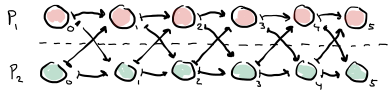
\includegraphics[scale=0.7]{images/product.png}
\caption{Illustration of a product of two processes. The process holds components of both states and applies the step function to both components simultaneously. To understand why the components have two incoming arrows, we need to discuss policies. A policy for a product process has access to both states and computes controls for both components. Thus it can base the choice of control for one component on both state components.}
\label{images:product}
\end{figure}

%
With the product combinator now at hand we illustrate how we can use it.
%
We apply the combinator to the system assumed to exist earlier.
%
\begin{hscode}\SaveRestoreHook
\column{B}{@{}>{\hspre}l<{\hspost}@{}}%
\column{E}{@{}>{\hspre}l<{\hspost}@{}}%
\>[B]{}\Varid{2d\text{-}system}\;\mathrel{=}\;\Varid{1\!d\text{-}sys}\;×_{\!\Varid{SDP}}\;\Varid{1\!d\text{-}sys}{}\<[E]%
\ColumnHook
\end{hscode}\resethooks
%
Now \ensuremath{\Varid{2d\text{-}system}} is a process of two dimensions rather than one, as illustrated by the type of \ensuremath{\Varid{test2}}.
%
To reuse the policy sequence we need to also combine policies, which we show how to do in section \ref{subsec:policycombinators} of the appendix.
%
\begin{hscode}\SaveRestoreHook
\column{B}{@{}>{\hspre}l<{\hspost}@{}}%
\column{14}{@{}>{\hspre}l<{\hspost}@{}}%
\column{16}{@{}>{\hspre}l<{\hspost}@{}}%
\column{19}{@{}>{\hspre}l<{\hspost}@{}}%
\column{50}{@{}>{\hspre}l<{\hspost}@{}}%
\column{E}{@{}>{\hspre}l<{\hspost}@{}}%
\>[B]{}\Varid{2d\text{-}pseq}\;\mathrel{=}\;\Varid{zipWith}\;\unopun{\mathop{×_{\!\Varid{P}}}}\;\Varid{pseq}\;\Varid{pseq}{}\<[E]%
\\
\>[B]{}\Varid{2d\text{-}test1}\;\mathbin{:}\;{}\<[14]%
\>[14]{}\Varid{trajectory}\;\Varid{2d\text{-}system}\;\Varid{2d\text{-}pseq}\;(\Varid{0}\;\Varid{,}\;\Varid{5})\;{}\<[E]%
\\
\>[14]{}\hsindent{2}{}\<[16]%
\>[16]{}\Varid{≡}\;{}\<[19]%
\>[19]{}(\Varid{0}\;\Varid{,}\;\Varid{4})\;\Varid{∷}\;(\Varid{0}\;\Varid{,}\;\Varid{3})\;\Varid{∷}\;(\Varid{1}\;\Varid{,}\;\Varid{4})\;\Varid{∷}\;{}\<[50]%
\>[50]{}(\Varid{1}\;\Varid{,}\;\Varid{4})\;\Varid{∷}\;(\Varid{2}\;\Varid{,}\;\Varid{5})\;\Varid{∷}\;\Varid{[]}{}\<[E]%
\\
\>[B]{}\Varid{2d\text{-}test1}\;\mathrel{=}\;\Varid{refl}{}\<[E]%
\ColumnHook
\end{hscode}\resethooks
%
Further work is presented in the appendix.
%
We present more combinators both for time dependent and time independent processes.
%
We implement the example of a coordinate system described above, and make it even more precise as a time dependent process.
%

% \paragraph{Acknowledgements.}
% %
% The reviewers suggested many improvements to the paper.

%------------------------------------------------------------------------------
%\newpage
\bibliography{paper}

\clearpage
\appendix
\section{Appendix}
\label{sec:appendix}
\TODO{Better title perhaps}
\subsection{Project introduction}
\label{subsec:projectintroduction}
\TODO{Är det GU + Chalmers? Jag vet aldrig hur jag skall framställa sådant här pga sammmarbetet.}
%
The work described in this text is the result of a project carried out at Gothenburg University by Robert Krook, under the supervision of Patrik Jansson.
%
Robert has worked independently and met once a week with Patrik over the course of 8 weeks to discuss progress, potential bottlenecks and what to do next.
%
Patrik has been an invaluable source of information, both regarding sequential decision problems and how to write a scientific text.
%
% -*- latex -*-

\subsection{Example}
\label{subsec:example}


Let us consider a sequential decision process where the state space is a one dimensional coordinate system represented by natural numbers.
%
\begin{hscode}\SaveRestoreHook
\column{B}{@{}>{\hspre}l<{\hspost}@{}}%
\column{13}{@{}>{\hspre}l<{\hspost}@{}}%
\column{16}{@{}>{\hspre}l<{\hspost}@{}}%
\column{E}{@{}>{\hspre}l<{\hspost}@{}}%
\>[B]{}\Varid{1\!d\text{-}state}\;{}\<[13]%
\>[13]{}\mathbin{:}\;{}\<[16]%
\>[16]{}\Conid{Set}{}\<[E]%
\\
\>[B]{}\Varid{1\!d\text{-}state}\;{}\<[13]%
\>[13]{}\mathrel{=}\;{}\<[16]%
\>[16]{}\Conid{ℕ}{}\<[E]%
\ColumnHook
\end{hscode}\resethooks


%
Seeing how the state space are the natural numbers we emphasize that the coordinate system has only positive coordinates.
%
In any given state, generally, we can choose to either increment, decrement or do nothing to the state.
%
In the edge case where the state is \ensuremath{\Varid{0}} we can not decrement the state.
%
We can encode this control as a type family in Agda.
%
\begin{hscode}\SaveRestoreHook
\column{B}{@{}>{\hspre}l<{\hspost}@{}}%
\column{3}{@{}>{\hspre}l<{\hspost}@{}}%
\column{10}{@{}>{\hspre}l<{\hspost}@{}}%
\column{E}{@{}>{\hspre}l<{\hspost}@{}}%
\>[B]{}\mathbf{data}\;\Varid{1d\text{-}control}\;\mathbin{:}\;\Varid{1\!d\text{-}state}\;\to \;\Conid{Set}\;\mathbf{where}{}\<[E]%
\\
\>[B]{}\hsindent{3}{}\<[3]%
\>[3]{}\Conid{Right}\;{}\<[10]%
\>[10]{}\mathbin{:}\;\{\mskip1.5mu \Varid{n}\;\mathbin{:}\;\Varid{1\!d\text{-}state}\mskip1.5mu\}\;\to \;\Varid{1d\text{-}control}\;\Varid{n}{}\<[E]%
\\
\>[B]{}\hsindent{3}{}\<[3]%
\>[3]{}\Conid{Stay}\;{}\<[10]%
\>[10]{}\mathbin{:}\;\{\mskip1.5mu \Varid{n}\;\mathbin{:}\;\Varid{1\!d\text{-}state}\mskip1.5mu\}\;\to \;\Varid{1d\text{-}control}\;\Varid{n}{}\<[E]%
\\
\>[B]{}\hsindent{3}{}\<[3]%
\>[3]{}\Conid{Left}\;{}\<[10]%
\>[10]{}\mathbin{:}\;\{\mskip1.5mu \Varid{n}\;\mathbin{:}\;\Varid{1\!d\text{-}state}\mskip1.5mu\}\;\to \;\Varid{1d\text{-}control}\;(\Varid{suc}\;\Varid{n}){}\<[E]%
\ColumnHook
\end{hscode}\resethooks
%
We implement the step function by pattern matching on the control.
%
\TODO{spellcheck recognises}
In the case of the \ensuremath{\Conid{Left}} control Agda recognises that the state must be a sucessor.
%
We increment or decrement the state accordingly and leave it unchanged for the \ensuremath{\Conid{Stay}} control.
%
\begin{hscode}\SaveRestoreHook
\column{B}{@{}>{\hspre}l<{\hspost}@{}}%
\column{12}{@{}>{\hspre}l<{\hspost}@{}}%
\column{15}{@{}>{\hspre}l<{\hspost}@{}}%
\column{20}{@{}>{\hspre}l<{\hspost}@{}}%
\column{27}{@{}>{\hspre}l<{\hspost}@{}}%
\column{E}{@{}>{\hspre}l<{\hspost}@{}}%
\>[B]{}\Varid{1d\text{-}step}\;{}\<[12]%
\>[12]{}\mathbin{:}\;{}\<[15]%
\>[15]{}(\Varid{x}\;\mathbin{:}\;\Varid{1\!d\text{-}state})\;\to \;\Varid{1d\text{-}control}\;\Varid{x}\;\to \;\Varid{1\!d\text{-}state}{}\<[E]%
\\
\>[B]{}\Varid{1d\text{-}step}\;\Varid{x}\;{}\<[20]%
\>[20]{}\Conid{Right}\;{}\<[27]%
\>[27]{}\mathrel{=}\;\Varid{suc}\;\Varid{x}{}\<[E]%
\\
\>[B]{}\Varid{1d\text{-}step}\;\Varid{x}\;{}\<[20]%
\>[20]{}\Conid{Stay}\;{}\<[27]%
\>[27]{}\mathrel{=}\;\Varid{x}{}\<[E]%
\\
\>[B]{}\Varid{1d\text{-}step}\;(\Varid{suc}\;\Varid{x})\;{}\<[20]%
\>[20]{}\Conid{Left}\;{}\<[27]%
\>[27]{}\mathrel{=}\;\Varid{x}{}\<[E]%
\ColumnHook
\end{hscode}\resethooks
%
We define a policy to be a function that given a state select a control.
%
The policies right, stay and tryleft are all policies of this kind.
%
tryleft is special in the sense that if the state is zero it will do nothing, as it can not go left.
%
\TODO{Put policy in record}
\begin{hscode}\SaveRestoreHook
\column{B}{@{}>{\hspre}l<{\hspost}@{}}%
\column{10}{@{}>{\hspre}l<{\hspost}@{}}%
\column{19}{@{}>{\hspre}l<{\hspost}@{}}%
\column{E}{@{}>{\hspre}l<{\hspost}@{}}%
\>[B]{}\Varid{1\!d\text{-}Policy}\;\mathrel{=}\;(\Varid{x}\;\mathbin{:}\;\Varid{1\!d\text{-}state})\;\to \;\Varid{1d\text{-}control}\;\Varid{x}{}\<[E]%
\\[\blanklineskip]%
\>[B]{}\Varid{right}\;\Varid{stay}\;\Varid{tryleft}\;\mathbin{:}\;\Varid{1\!d\text{-}Policy}{}\<[E]%
\\
\>[B]{}\Varid{right}\;{}\<[10]%
\>[10]{}\anonymous \;{}\<[19]%
\>[19]{}\mathrel{=}\;\Conid{Right}{}\<[E]%
\\
\>[B]{}\Varid{stay}\;{}\<[10]%
\>[10]{}\anonymous \;{}\<[19]%
\>[19]{}\mathrel{=}\;\Conid{Stay}{}\<[E]%
\\
\>[B]{}\Varid{tryleft}\;{}\<[10]%
\>[10]{}\Varid{zero}\;{}\<[19]%
\>[19]{}\mathrel{=}\;\Conid{Stay}{}\<[E]%
\\
\>[B]{}\Varid{tryleft}\;{}\<[10]%
\>[10]{}(\Varid{suc}\;\Varid{s})\;{}\<[19]%
\>[19]{}\mathrel{=}\;\Conid{Left}{}\<[E]%
\ColumnHook
\end{hscode}\resethooks
%
We can parameterise a policy over a coordinate and define a policy that will select controls that moves the system towards this coordinate.
%
\begin{hscode}\SaveRestoreHook
\column{B}{@{}>{\hspre}l<{\hspost}@{}}%
\column{20}{@{}>{\hspre}l<{\hspost}@{}}%
\column{E}{@{}>{\hspre}l<{\hspost}@{}}%
\>[B]{}\Varid{towards}\;\mathbin{:}\;\Conid{ℕ}\;\to \;\Varid{1\!d\text{-}Policy}{}\<[E]%
\\
\>[B]{}\Varid{towards}\;\Varid{goal}\;\Varid{n}\;\mathbf{with}\;\Varid{compare}\;\Varid{n}\;\Varid{goal}{}\<[E]%
\\
\>[B]{}\Varid{...}\;\mid \;\Varid{less}\;\anonymous \;\anonymous \;{}\<[20]%
\>[20]{}\mathrel{=}\;\Conid{Right}{}\<[E]%
\\
\>[B]{}\Varid{...}\;\mid \;\Varid{equal}\;\anonymous \;{}\<[20]%
\>[20]{}\mathrel{=}\;\Conid{Stay}{}\<[E]%
\\
\>[B]{}\Varid{...}\;\mid \;\Varid{greater}\;\anonymous \;\anonymous \;{}\<[20]%
\>[20]{}\mathrel{=}\;\Conid{Left}{}\<[E]%
\ColumnHook
\end{hscode}\resethooks
%
With the three components state, control and step, we can instantiate a sequential decision process.
%
\begin{hscode}\SaveRestoreHook
\column{B}{@{}>{\hspre}l<{\hspost}@{}}%
\column{14}{@{}>{\hspre}l<{\hspost}@{}}%
\column{17}{@{}>{\hspre}l<{\hspost}@{}}%
\column{E}{@{}>{\hspre}l<{\hspost}@{}}%
\>[B]{}\Varid{1\!d\text{-}sys}\;{}\<[14]%
\>[14]{}\mathbin{:}\;{}\<[17]%
\>[17]{}\Conid{SDProc}{}\<[E]%
\\
\>[B]{}\Varid{1\!d\text{-}sys}\;{}\<[14]%
\>[14]{}\mathrel{=}\;{}\<[17]%
\>[17]{}\Conid{SDP}\;\Varid{1\!d\text{-}state}\;\Varid{1d\text{-}control}\;\Varid{1d\text{-}step}{}\<[E]%
\ColumnHook
\end{hscode}\resethooks
%
A policy sequence is now just a vector of policies.
%
\begin{hscode}\SaveRestoreHook
\column{B}{@{}>{\hspre}l<{\hspost}@{}}%
\column{E}{@{}>{\hspre}l<{\hspost}@{}}%
\>[B]{}\Varid{pseq}\;\mathbin{:}\;\Conid{PolicySeq}\;(\Varid{\#}\ensuremath{_{\text{st}}}\;\Varid{1\!d\text{-}sys})\;(\Varid{\#}\ensuremath{_{\text{c}}}\;\Varid{1\!d\text{-}sys})\;\Varid{5}{}\<[E]%
\\
\>[B]{}\Varid{pseq}\;\mathrel{=}\;\Varid{tryleft}\;\Varid{∷}\;\Varid{tryleft}\;\Varid{∷}\;\Varid{right}\;\Varid{∷}\;\Varid{stay}\;\Varid{∷}\;\Varid{right}\;\Varid{∷}\;\Varid{[]}{}\<[E]%
\ColumnHook
\end{hscode}\resethooks
%
We can evaluate the system using this sequence, starting from different points.
%
We can use \ensuremath{\Varid{≡}} and \ensuremath{\Varid{refl}} to assert that the system behaves as intended.
%\TODO{Maybe explain briefly what refl and ≡ are?}
%
\begin{hscode}\SaveRestoreHook
\column{B}{@{}>{\hspre}l<{\hspost}@{}}%
\column{42}{@{}>{\hspre}l<{\hspost}@{}}%
\column{E}{@{}>{\hspre}l<{\hspost}@{}}%
\>[B]{}\Varid{test1}\;\mathbin{:}\;\Varid{trajectory}\;\Varid{1\!d\text{-}sys}\;\Varid{pseq}\;\Varid{0}\;\Varid{≡}\;{}\<[42]%
\>[42]{}\Varid{0}\;\Varid{∷}\;\Varid{0}\;\Varid{∷}\;\Varid{1}\;\Varid{∷}\;{}\<[E]%
\\
\>[42]{}\Varid{1}\;\Varid{∷}\;\Varid{2}\;\Varid{∷}\;\Varid{[]}{}\<[E]%
\\
\>[B]{}\Varid{test1}\;\mathrel{=}\;\Varid{refl}{}\<[E]%
\\[\blanklineskip]%
\>[B]{}\Varid{test2}\;\mathbin{:}\;\Varid{trajectory}\;\Varid{1\!d\text{-}sys}\;\Varid{pseq}\;\Varid{5}\;\Varid{≡}\;{}\<[42]%
\>[42]{}\Varid{4}\;\Varid{∷}\;\Varid{3}\;\Varid{∷}\;\Varid{4}\;\Varid{∷}\;{}\<[E]%
\\
\>[42]{}\Varid{4}\;\Varid{∷}\;\Varid{5}\;\Varid{∷}\;\Varid{[]}{}\<[E]%
\\
\>[B]{}\Varid{test2}\;\mathrel{=}\;\Varid{refl}{}\<[E]%
\ColumnHook
\end{hscode}\resethooks
%
We can use the clever policy to steer the process towards a goal.
%
\begin{hscode}\SaveRestoreHook
\column{B}{@{}>{\hspre}l<{\hspost}@{}}%
\column{10}{@{}>{\hspre}l<{\hspost}@{}}%
\column{11}{@{}>{\hspre}l<{\hspost}@{}}%
\column{E}{@{}>{\hspre}l<{\hspost}@{}}%
\>[B]{}\Varid{test3}\;\mathbin{:}\;{}\<[10]%
\>[10]{}\Varid{trajectory}\;\Varid{1\!d\text{-}sys}\;(\Varid{replicate}\;(\Varid{towards}\;\Varid{5}))\;\Varid{2}\;\Varid{≡}\;{}\<[E]%
\\
\>[10]{}\hsindent{1}{}\<[11]%
\>[11]{}\Varid{3}\;\Varid{∷}\;\Varid{4}\;\Varid{∷}\;\Varid{5}\;\Varid{∷}\;\Varid{5}\;\Varid{∷}\;\Varid{5}\;\Varid{∷}\;\Varid{[]}{}\<[E]%
\\
\>[B]{}\Varid{test3}\;\mathrel{=}\;\Varid{refl}{}\<[E]%
\ColumnHook
\end{hscode}\resethooks

%
To turn a process into a problem we need to introduce a notion of a goal, described by a \ensuremath{\Varid{reward}} function.
%
For our example we define the reward function to be parameterised over a target coordinate.
%
The reward function could then reward a proposed step based on how close to the target it lands.
%
\begin{hscode}\SaveRestoreHook
\column{B}{@{}>{\hspre}l<{\hspost}@{}}%
\column{3}{@{}>{\hspre}l<{\hspost}@{}}%
\column{5}{@{}>{\hspre}l<{\hspost}@{}}%
\column{11}{@{}>{\hspre}l<{\hspost}@{}}%
\column{14}{@{}>{\hspre}l<{\hspost}@{}}%
\column{17}{@{}>{\hspre}l<{\hspost}@{}}%
\column{E}{@{}>{\hspre}l<{\hspost}@{}}%
\>[B]{}\Varid{1d\text{-}reward}\;{}\<[14]%
\>[14]{}\mathbin{:}\;{}\<[17]%
\>[17]{}\Varid{1\!d\text{-}state}\;{}\<[E]%
\\
\>[14]{}\Varid{→}\;{}\<[17]%
\>[17]{}(\Varid{x}\;\mathbin{:}\;\Varid{1\!d\text{-}state})\;\Varid{→}\;\Varid{1d\text{-}control}\;\Varid{x}\;{}\<[E]%
\\
\>[14]{}\Varid{→}\;{}\<[17]%
\>[17]{}\Varid{1\!d\text{-}state}\;\Varid{→}\;\Conid{ℕ}{}\<[E]%
\\
\>[B]{}\Varid{1d\text{-}reward}\;\Varid{target}\;\Varid{x₀}\;\Varid{y}\;\Varid{x₁}\;{}\<[E]%
\\
\>[B]{}\hsindent{3}{}\<[3]%
\>[3]{}\mathrel{=}\;\Varid{if}\;\Varid{distance}\;\Varid{target}\;\Varid{x₁}\;\Varid{<}\;\Varid{distance}\;\Varid{target}\;\Varid{x₀}\;{}\<[E]%
\\
\>[3]{}\hsindent{2}{}\<[5]%
\>[5]{}\Varid{then}\;\Varid{2}\;{}\<[E]%
\\
\>[3]{}\hsindent{2}{}\<[5]%
\>[5]{}\Varid{else}\;(\Varid{if}\;\Varid{distance}\;\Varid{target}\;\Varid{x₀}\;\Varid{<}\;\Varid{distance}\;\Varid{target}\;\Varid{x₁}{}\<[E]%
\\
\>[5]{}\hsindent{6}{}\<[11]%
\>[11]{}\Varid{then}\;\Varid{0}{}\<[E]%
\\
\>[5]{}\hsindent{6}{}\<[11]%
\>[11]{}\Varid{else}\;\Varid{1}){}\<[E]%
\ColumnHook
\end{hscode}\resethooks
%
We can redefine the sequential decision process above to be a sequential decision problem simply by instantiating the \ensuremath{\Conid{SDProb}} record.
%
\begin{hscode}\SaveRestoreHook
\column{B}{@{}>{\hspre}l<{\hspost}@{}}%
\column{3}{@{}>{\hspre}l<{\hspost}@{}}%
\column{13}{@{}>{\hspre}l<{\hspost}@{}}%
\column{25}{@{}>{\hspre}l<{\hspost}@{}}%
\column{E}{@{}>{\hspre}l<{\hspost}@{}}%
\>[B]{}\Varid{problem}\;\mathbin{:}\;\Varid{1\!d\text{-}state}\;\to \;\Conid{SDProblem}{}\<[E]%
\\
\>[B]{}\Varid{problem}\;\Varid{target}\;{}\<[E]%
\\
\>[B]{}\hsindent{3}{}\<[3]%
\>[3]{}\mathrel{=}\;\Conid{SDProb}\;{}\<[13]%
\>[13]{}\Varid{1\!d\text{-}state}\;{}\<[25]%
\>[25]{}\Varid{1d\text{-}control}\;{}\<[E]%
\\
\>[13]{}\Varid{1d\text{-}step}\;{}\<[25]%
\>[25]{}(\Varid{1d\text{-}reward}\;\Varid{target}){}\<[E]%
\ColumnHook
\end{hscode}\resethooks

%\TODO{Example ``run'' would be instructive}
%------------------------------------------------------------------------------
% -*- latex -*-
\subsection{Combinators for sequential decision processes}
\label{subsec:combsecdecproc}


%
Now that we've seen an example of a sequential decision process and are getting comfortable with the concept, it is suitable to move forward and see what we can do with processes.
%
This section will explore different ways sequential decision processes can be combined in order to produce more sophisticated processes.
%
%-----------------------------------------------------------------------

%
We already defined the product combinator, and before we move on to additional combinators we'd like to make a few notes on the product combinator.
%
An observation to be made is that in order for the new system to exist in any state, it has to hold components of both prior states.
%
This has the consequence that if the state space of one of the prior processes is empty, the new problems state space is also empty.
%
Similarly, if one of the components reaches a point where there are no available controls, and thus can not progress, the other component will not be able to progress either.
%

% -*- latex -*-

%
Looking back at the example of the one dimensional coordinate system we find ourselves wondering if we would now indeed get a process of a two dimensional coordinate system seemingly for free.
%
The answer, unsurprisingly, is yes.
%
\begin{hscode}\SaveRestoreHook
\column{B}{@{}>{\hspre}l<{\hspost}@{}}%
\column{E}{@{}>{\hspre}l<{\hspost}@{}}%
\>[B]{}\Varid{2d\text{-}system}\;\mathrel{=}\;\Varid{1\!d\text{-}sys}\;×_{\!\Varid{SDP}}\;\Varid{1\!d\text{-}sys}{}\<[E]%
\ColumnHook
\end{hscode}\resethooks

%
In section \ref{subsec:policycombinators} we introduce combinators for policy sequences.
%
Here we use the product combinator to produce a policy sequence that is compatible with the new process.
%
\begin{hscode}\SaveRestoreHook
\column{B}{@{}>{\hspre}l<{\hspost}@{}}%
\column{17}{@{}>{\hspre}l<{\hspost}@{}}%
\column{E}{@{}>{\hspre}l<{\hspost}@{}}%
\>[B]{}\Varid{2d\text{-}pseq}\;\mathbin{:}\;{}\<[17]%
\>[17]{}\Conid{PolicySeq}\;(\Varid{\#}\ensuremath{_{\text{st}}}\;\Varid{2d\text{-}system})\;(\Varid{\#}\ensuremath{_{\text{c}}}\;\Varid{2d\text{-}system})\;\Varid{5}{}\<[E]%
\\
\>[B]{}\Varid{2d\text{-}pseq}\;\mathrel{=}\;{}\<[17]%
\>[17]{}\Varid{zipWith}\;\unopun{\mathop{×_{\!\Varid{P}}}}\;\Varid{pseq}\;\Varid{pseq}{}\<[E]%
\ColumnHook
\end{hscode}\resethooks
%
And now we can evaluate this new process like we did with the one dimensional system.
%
\begin{hscode}\SaveRestoreHook
\column{B}{@{}>{\hspre}l<{\hspost}@{}}%
\column{14}{@{}>{\hspre}l<{\hspost}@{}}%
\column{E}{@{}>{\hspre}l<{\hspost}@{}}%
\>[B]{}\Varid{run2d}\;\mathrel{=}\;\Varid{trajectory}\;\Varid{2d\text{-}system}\;\Varid{2d\text{-}pseq}{}\<[E]%
\\[\blanklineskip]%
\>[B]{}\Varid{2d\text{-}test1}\;\mathbin{:}\;{}\<[14]%
\>[14]{}\Varid{run2d}\;(\Varid{0}\;\Varid{,}\;\Varid{5})\;{}\<[E]%
\\
\>[14]{}\Varid{≡}\;{}\<[E]%
\\
\>[14]{}(\Varid{0}\;\Varid{,}\;\Varid{4})\;\Varid{∷}\;(\Varid{0}\;\Varid{,}\;\Varid{3})\;\Varid{∷}\;(\Varid{1}\;\Varid{,}\;\Varid{4})\;\Varid{∷}\;{}\<[E]%
\\
\>[14]{}(\Varid{1}\;\Varid{,}\;\Varid{4})\;\Varid{∷}\;(\Varid{2}\;\Varid{,}\;\Varid{5})\;\Varid{∷}\;(\Varid{2}\;\Varid{,}\;\Varid{5})\;\Varid{∷}\;\Varid{[]}{}\<[E]%
\\
\>[B]{}\Varid{2d\text{-}test1}\;\mathrel{=}\;\Varid{refl}{}\<[E]%
\\[\blanklineskip]%
\>[B]{}\Varid{2d\text{-}test2}\;\mathbin{:}\;{}\<[14]%
\>[14]{}\Varid{run2d}\;(\Varid{5}\;\Varid{,}\;\Varid{5})\;{}\<[E]%
\\
\>[14]{}\Varid{≡}\;{}\<[E]%
\\
\>[14]{}(\Varid{4}\;\Varid{,}\;\Varid{4})\;\Varid{∷}\;(\Varid{3}\;\Varid{,}\;\Varid{3})\;\Varid{∷}\;(\Varid{4}\;\Varid{,}\;\Varid{4})\;\Varid{∷}\;{}\<[E]%
\\
\>[14]{}(\Varid{4}\;\Varid{,}\;\Varid{4})\;\Varid{∷}\;(\Varid{5}\;\Varid{,}\;\Varid{5})\;\Varid{∷}\;(\Varid{5}\;\Varid{,}\;\Varid{5})\;\Varid{∷}\;\Varid{[]}{}\<[E]%
\\
\>[B]{}\Varid{2d\text{-}test2}\;\mathrel{=}\;\Varid{refl}{}\<[E]%
\ColumnHook
\end{hscode}\resethooks

%
Functional programmers will often find they are in need of a unit, e.g when using \ensuremath{\Varid{reduce}} or other frequently appearing constructs from the functional paradigm.
%
Before we begin implementing a unit for the product case we want to clarify what we mean by a unit.
%
A unit to a process is one that when combined with another process, produces a process where the change at each step is exactly that of the other process.
%

%
What we are after is a process that will not carry any extra information, or rather one that can not alter the information it carries.
%
Recall that in order for the state space of the product process to not be empty, both state spaces of the separate processes has to be non-empty.
%
In order to call the step function the control space also has to be inhabited.
%
In an effort to minimise the information the unit carries we declare its state space and control space to be singletons.
%
The step function becomes a constant function that given the only state and the only control, will return the only state.
%
\begin{hscode}\SaveRestoreHook
\column{B}{@{}>{\hspre}l<{\hspost}@{}}%
\column{3}{@{}>{\hspre}l<{\hspost}@{}}%
\column{12}{@{}>{\hspre}l<{\hspost}@{}}%
\column{15}{@{}>{\hspre}l<{\hspost}@{}}%
\column{E}{@{}>{\hspre}l<{\hspost}@{}}%
\>[B]{}\Varid{singleton}\;\mathbin{:}\;\Conid{SDProc}{}\<[E]%
\\
\>[B]{}\Varid{singleton}\;\mathrel{=}\;\mathbf{record}\;\{\mskip1.5mu {}\<[E]%
\\
\>[B]{}\hsindent{3}{}\<[3]%
\>[3]{}\Conid{State}\;{}\<[12]%
\>[12]{}\mathrel{=}\;{}\<[15]%
\>[15]{}\Varid{⊤};{}\<[E]%
\\
\>[B]{}\hsindent{3}{}\<[3]%
\>[3]{}\Conid{Control}\;{}\<[12]%
\>[12]{}\mathrel{=}\;{}\<[15]%
\>[15]{}\lambda\;\Varid{state}\;\to \;\Varid{⊤};{}\<[E]%
\\
\>[B]{}\hsindent{3}{}\<[3]%
\>[3]{}\Varid{step}\;{}\<[12]%
\>[12]{}\mathrel{=}\;{}\<[15]%
\>[15]{}\lambda\;\Varid{state}\;\to \;\lambda\;\Varid{control}\;\to \;\Varid{tt}\mskip1.5mu\}{}\<[E]%
\ColumnHook
\end{hscode}\resethooks
%
An example of evaluating the singleton process is illustrated in Figure \ref{images:singleton}
%
\begin{figure}
\centering
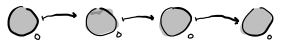
\includegraphics[scale=0.7]{images/singleton.png}
\caption{Illustration of the singleton process. The subscript ₀ is meant to indicate that the state remains the same when the process advances.}
\label{images:singleton}
\end{figure}

%
Taking the product of any process and the singleton process would produce a process where the only change of information during each step is that of the process which is not the singleton.
%
Of course, the other process could itself be the singleton process also, in which case the only change in each step is exactly that of the singleton process, which is no change at all.
%

%-----------------------------------------------------------------------
\subsubsection{Coproduct}
\label{subsubsec:coproductseqdecproc}

%
Seeing how we defined a product combinator of two processes, we are interested in also defining a sum combinator for processes.
%
The approach is similar to that of the product case.
%

%
The inhabitants of the sum control is the sum of the inhabitants of the prior controls.
%
\begin{hscode}\SaveRestoreHook
\column{B}{@{}>{\hspre}l<{\hspost}@{}}%
\column{7}{@{}>{\hspre}l<{\hspost}@{}}%
\column{10}{@{}>{\hspre}l<{\hspost}@{}}%
\column{23}{@{}>{\hspre}l<{\hspost}@{}}%
\column{E}{@{}>{\hspre}l<{\hspost}@{}}%
\>[B]{}\unopun{⊎_{\!\Varid{C}}}\;{}\<[7]%
\>[7]{}\mathbin{:}\;{}\<[10]%
\>[10]{}\{\mskip1.5mu \Conid{S₁}\;\Conid{S₂}\;\mathbin{:}\;\Conid{Set}\mskip1.5mu\}\;{}\<[E]%
\\
\>[7]{}\Varid{→}\;{}\<[10]%
\>[10]{}\Conid{Con}\;\Conid{S₁}\;\Varid{→}\;\Conid{Con}\;\Conid{S₂}\;\Varid{→}\;\Conid{Con}\;(\Conid{S₁}\;\Varid{⊎}\;\Conid{S₂}){}\<[E]%
\\
\>[B]{}(\Conid{C₁}\;⊎_{\!\Varid{C}}\;\Conid{C₂})\;(\Varid{inj₁}\;\Varid{s₁})\;{}\<[23]%
\>[23]{}\mathrel{=}\;\Conid{C₁}\;\Varid{s₁}{}\<[E]%
\\
\>[B]{}(\Conid{C₁}\;⊎_{\!\Varid{C}}\;\Conid{C₂})\;(\Varid{inj₂}\;\Varid{s₂})\;{}\<[23]%
\>[23]{}\mathrel{=}\;\Conid{C₂}\;\Varid{s₂}{}\<[E]%
\ColumnHook
\end{hscode}\resethooks
%
Calculating a new step function from two prior step functions is relatively straight forward.
%
The first input is the sum of the two states.
%
Depending on which state the first argument belongs to, one of the prior step functions is applied to it and the second argument, the control for that state.
%
The result of the application is then injected into the sum type using the same injection as the input.
%
\begin{hscode}\SaveRestoreHook
\column{B}{@{}>{\hspre}l<{\hspost}@{}}%
\column{8}{@{}>{\hspre}l<{\hspost}@{}}%
\column{12}{@{}>{\hspre}l<{\hspost}@{}}%
\column{29}{@{}>{\hspre}l<{\hspost}@{}}%
\column{E}{@{}>{\hspre}l<{\hspost}@{}}%
\>[B]{}\unopun{⊎_{\!\Varid{sf}}}\;{}\<[8]%
\>[8]{}\mathbin{:}\;{}\<[12]%
\>[12]{}\{\mskip1.5mu \Conid{S₁}\;\Conid{S₂}\;\mathbin{:}\;\Conid{Set}\mskip1.5mu\}\;{}\<[E]%
\\
\>[8]{}\to \;{}\<[12]%
\>[12]{}\{\mskip1.5mu \Conid{C₁}\;\mathbin{:}\;\Conid{Con}\;\Conid{S₁}\mskip1.5mu\}\;\to \;\{\mskip1.5mu \Conid{C₂}\;\mathbin{:}\;\Conid{Con}\;\Conid{S₂}\mskip1.5mu\}\;{}\<[E]%
\\
\>[8]{}\to \;{}\<[12]%
\>[12]{}\Conid{Step}\;\Conid{S₁}\;\Conid{C₁}\;\to \;\Conid{Step}\;\Conid{S₂}\;\Conid{C₂}\;{}\<[E]%
\\
\>[8]{}\to \;{}\<[12]%
\>[12]{}\Conid{Step}\;(\Conid{S₁}\;\Varid{⊎}\;\Conid{S₂})\;(\Conid{C₁}\;⊎_{\!\Varid{C}}\;\Conid{C₂}){}\<[E]%
\\
\>[B]{}(\Varid{sf₁}\;⊎_{\!\Varid{sf}}\;\Varid{sf₂})\;(\Varid{inj₁}\;\Varid{s₁})\;\Varid{c₁}\;{}\<[29]%
\>[29]{}\mathrel{=}\;\Varid{inj₁}\;(\Varid{sf₁}\;\Varid{s₁}\;\Varid{c₁}){}\<[E]%
\\
\>[B]{}(\Varid{sf₁}\;⊎_{\!\Varid{sf}}\;\Varid{sf₂})\;(\Varid{inj₂}\;\Varid{s₂})\;\Varid{c₂}\;{}\<[29]%
\>[29]{}\mathrel{=}\;\Varid{inj₂}\;(\Varid{sf₂}\;\Varid{s₂}\;\Varid{c₂}){}\<[E]%
\ColumnHook
\end{hscode}\resethooks
%
The sum of two problems is computed by applying the sum operators componentwise, and Figure \ref{images:coproduct} illustrate how such a problem is evaluated.
%
\begin{hscode}\SaveRestoreHook
\column{B}{@{}>{\hspre}l<{\hspost}@{}}%
\column{3}{@{}>{\hspre}l<{\hspost}@{}}%
\column{E}{@{}>{\hspre}l<{\hspost}@{}}%
\>[B]{}\unopun{⊎_{\!\Varid{SDP}}}\;\mathbin{:}\;\Conid{SDProc}\;\Varid{→}\;\Conid{SDProc}\;\Varid{→}\;\Conid{SDProc}{}\<[E]%
\\
\>[B]{}\Conid{SDP}\;\Conid{S₁}\;\Conid{C₁}\;\Varid{sf₁}\;⊎_{\!\Varid{SDP}}\;\Conid{SDP}\;\Conid{S₂}\;\Conid{C₂}\;\Varid{sf₂}\;{}\<[E]%
\\
\>[B]{}\hsindent{3}{}\<[3]%
\>[3]{}\mathrel{=}\;\Conid{SDP}\;(\Conid{S₁}\;\Varid{⊎}\;\Conid{S₂})\;(\Conid{C₁}\;⊎_{\!\Varid{C}}\;\Conid{C₂})\;(\Varid{sf₁}\;⊎_{\!\Varid{sf}}\;\Varid{sf₂}){}\<[E]%
\ColumnHook
\end{hscode}\resethooks

\begin{figure}
\begin{subfigure}{.5\textwidth}
  \centering
  % include first image
  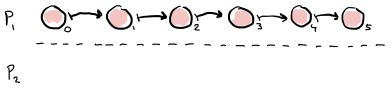
\includegraphics[width=.8\linewidth]{images/coproduct-inj1.png}
  \caption{Left injection.} % write better captions
  \label{images:coproduct-inj1}
\end{subfigure}
\begin{subfigure}{.5\textwidth}
  \centering
  % include second image
  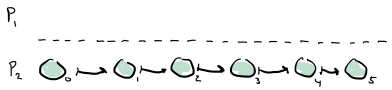
\includegraphics[width=.8\linewidth]{images/coproduct-inj2.png}
  \caption{Right injection.}
  \label{images:coproduct-inj2}
\end{subfigure}
\caption{The coproduct of two processes. The process will take the shape of either of the two alternatives, but never both or a mix of the two.}
\label{images:coproduct}
\end{figure}

%
In the case of the product process the two prior processes were not entirely independent.
%
If one process could not progress the other process was \emph{affected} in the sense that it too could not progress further.
%
The sum of two processes keeps the two problems truly independent.
%
In fact, the coproduct of two processes will start progressing from some initial state, and depending on which injection is used the other process will never advance.

%
A unit to the coproduct combinator is the empty process.
%
The process has no states, no controls and the step function will return its input state.
%
However, we will never be able to call the step function since we can not supply a state.
%
\begin{hscode}\SaveRestoreHook
\column{B}{@{}>{\hspre}l<{\hspost}@{}}%
\column{3}{@{}>{\hspre}l<{\hspost}@{}}%
\column{12}{@{}>{\hspre}l<{\hspost}@{}}%
\column{E}{@{}>{\hspre}l<{\hspost}@{}}%
\>[B]{}\Varid{empty}\;\mathbin{:}\;\Conid{SDProc}{}\<[E]%
\\
\>[B]{}\Varid{empty}\;\mathrel{=}\;\mathbf{record}\;\{\mskip1.5mu {}\<[E]%
\\
\>[B]{}\hsindent{3}{}\<[3]%
\>[3]{}\Conid{State}\;{}\<[12]%
\>[12]{}\mathrel{=}\;\Varid{⊥};{}\<[E]%
\\
\>[B]{}\hsindent{3}{}\<[3]%
\>[3]{}\Conid{Control}\;{}\<[12]%
\>[12]{}\mathrel{=}\;\lambda\;\Varid{state}\;\to \;\Varid{⊥};{}\<[E]%
\\
\>[B]{}\hsindent{3}{}\<[3]%
\>[3]{}\Varid{step}\;{}\<[12]%
\>[12]{}\mathrel{=}\;\lambda\;\Varid{state}\;\to \;\lambda\;\Varid{control}\;\to \;\Varid{state}\mskip1.5mu\}{}\<[E]%
\ColumnHook
\end{hscode}\resethooks

%
Combining any process with the empty process using the coproduct combinator will produce a process that acts exactly as that of the given process.
%
There is no way to begin advancing the empty process, and so the only available option is to select an initial state from the other process and start progressing that.
%

%-----------------------------------------------------------------------
\subsubsection{Yielding Coproduct}
\label{subsubsec:yieldingcoproductseqdecproc}

%
Computing the coproduct of two processes and getting a process that behaves like either of the two, without actually considering the other process, leaves us wondering what this is useful for.
%
It would be more useful if we could jump between the two processes.
%
To do this, we first need to define a relation between states.
%
We define a relation on two state and define it to be a mapping from an inhabitant of one state to an inhabitant of the other.
%
\begin{hscode}\SaveRestoreHook
\column{B}{@{}>{\hspre}l<{\hspost}@{}}%
\column{E}{@{}>{\hspre}l<{\hspost}@{}}%
\>[B]{}\unopun{\mathop{⇄}}\;\mathbin{:}\;(\Conid{S₁}\;\Conid{S₂}\;\mathbin{:}\;\Conid{Set})\;\Varid{→}\;\Conid{Set}{}\<[E]%
\\
\>[B]{}\Varid{s₁}\;\mathop{⇄}\;\Varid{s₂}\;\mathrel{=}\;(\Varid{s₁}\;\to \;\Varid{s₂})\;\Varid{×}\;(\Varid{s₂}\;\to \;\Varid{s₁}){}\<[E]%
\ColumnHook
\end{hscode}\resethooks
%
Combining the two controls on the states is similar to that of the coproduct case, when looking at the type.
%
However, instead of the new control being defined as either of the two prior ones, it is now \ensuremath{\Conid{Maybe}} either of the two previous ones.
%
The idea is that we extend the control space to have one more inhabitant, the value \ensuremath{\Varid{nothing}}.
%
If we select this control the process should yield in favour of the other process.
%
\begin{hscode}\SaveRestoreHook
\column{B}{@{}>{\hspre}l<{\hspost}@{}}%
\column{8}{@{}>{\hspre}l<{\hspost}@{}}%
\column{11}{@{}>{\hspre}l<{\hspost}@{}}%
\column{E}{@{}>{\hspre}l<{\hspost}@{}}%
\>[B]{}\unopun{⊎_{\!\Varid{C}}^m}\;{}\<[8]%
\>[8]{}\mathbin{:}\;{}\<[11]%
\>[11]{}\{\mskip1.5mu \Conid{S₁}\;\Conid{S₂}\;\mathbin{:}\;\Conid{Set}\mskip1.5mu\}\;{}\<[E]%
\\
\>[8]{}\Varid{→}\;{}\<[11]%
\>[11]{}\Conid{Con}\;\Conid{S₁}\;\Varid{→}\;\Conid{Con}\;\Conid{S₂}\;\Varid{→}\;\Conid{Con}\;(\Conid{S₁}\;\Varid{⊎}\;\Conid{S₂}){}\<[E]%
\\
\>[B]{}(\Conid{C₁}\;⊎_{\!\Varid{C}}^m\;\Conid{C₂})\;(\Varid{inj₁}\;\Varid{s₁})\;\mathrel{=}\;\Conid{Maybe}\;(\Conid{C₁}\;\Varid{s₁}){}\<[E]%
\\
\>[B]{}(\Conid{C₁}\;⊎_{\!\Varid{C}}^m\;\Conid{C₂})\;(\Varid{inj₂}\;\Varid{s₂})\;\mathrel{=}\;\Conid{Maybe}\;(\Conid{C₂}\;\Varid{s₂}){}\<[E]%
\ColumnHook
\end{hscode}\resethooks
%
The new step function needs to accomodate for this scenario where the process should yield in favour of the other.
%
To implement this the new step function needs to know \emph{how} to yield.
%
We describe how to yield by supplying an element of type \ensuremath{\Conid{S₁}\;\mathop{⇄}\;\Conid{S₂}}.
%
If the selected control is \ensuremath{\Varid{nothing}} the step function will apply the appropriate component of this element to the current state.
%
\begin{hscode}\SaveRestoreHook
\column{B}{@{}>{\hspre}l<{\hspost}@{}}%
\column{7}{@{}>{\hspre}l<{\hspost}@{}}%
\column{10}{@{}>{\hspre}l<{\hspost}@{}}%
\column{17}{@{}>{\hspre}l<{\hspost}@{}}%
\column{26}{@{}>{\hspre}l<{\hspost}@{}}%
\column{37}{@{}>{\hspre}l<{\hspost}@{}}%
\column{47}{@{}>{\hspre}l<{\hspost}@{}}%
\column{E}{@{}>{\hspre}l<{\hspost}@{}}%
\>[B]{}⊎_{\!\Varid{sf}}^m\;{}\<[7]%
\>[7]{}\mathbin{:}\;{}\<[10]%
\>[10]{}\{\mskip1.5mu \Conid{S₁}\;\Conid{S₂}\;\mathbin{:}\;\Conid{Set}\mskip1.5mu\}\;\{\mskip1.5mu \Conid{C₁}\;\mathbin{:}\;\Conid{Con}\;\Conid{S₁}\mskip1.5mu\}\;\{\mskip1.5mu \Conid{C₂}\;\mathbin{:}\;\Conid{Con}\;\Conid{S₂}\mskip1.5mu\}\;{}\<[E]%
\\
\>[7]{}\Varid{→}\;{}\<[10]%
\>[10]{}(\Conid{S₁}\;\mathop{⇄}\;\Conid{S₂})\;{}\<[E]%
\\
\>[7]{}\Varid{→}\;{}\<[10]%
\>[10]{}\Conid{Step}\;\Conid{S₁}\;\Conid{C₁}\;\Varid{→}\;\Conid{Step}\;\Conid{S₂}\;\Conid{C₂}\;{}\<[E]%
\\
\>[7]{}\Varid{→}\;{}\<[10]%
\>[10]{}\Conid{Step}\;(\Conid{S₁}\;\Varid{⊎}\;\Conid{S₂})\;(\Conid{C₁}\;⊎_{\!\Varid{C}}^m\;\Conid{C₂}){}\<[E]%
\\
\>[B]{}⊎_{\!\Varid{sf}}^m\;\anonymous \;{}\<[17]%
\>[17]{}\Varid{sf₁}\;\Varid{sf₂}\;{}\<[26]%
\>[26]{}(\Varid{inj₁}\;\Varid{s₁})\;{}\<[37]%
\>[37]{}(\Varid{just}\;\Varid{c})\;{}\<[47]%
\>[47]{}\mathrel{=}\;\Varid{inj₁}\;(\Varid{sf₁}\;\Varid{s₁}\;\Varid{c}){}\<[E]%
\\
\>[B]{}⊎_{\!\Varid{sf}}^m\;\anonymous \;{}\<[17]%
\>[17]{}\Varid{sf₁}\;\Varid{sf₂}\;{}\<[26]%
\>[26]{}(\Varid{inj₂}\;\Varid{s₂})\;{}\<[37]%
\>[37]{}(\Varid{just}\;\Varid{c})\;{}\<[47]%
\>[47]{}\mathrel{=}\;\Varid{inj₂}\;(\Varid{sf₂}\;\Varid{s₂}\;\Varid{c}){}\<[E]%
\\
\>[B]{}⊎_{\!\Varid{sf}}^m\;(\Varid{v₁}\;\Varid{,}\;\anonymous )\;{}\<[17]%
\>[17]{}\Varid{sf₁}\;\Varid{sf₂}\;{}\<[26]%
\>[26]{}(\Varid{inj₁}\;\Varid{s₁})\;{}\<[37]%
\>[37]{}\Varid{nothing}\;{}\<[47]%
\>[47]{}\mathrel{=}\;\Varid{inj₂}\;(\Varid{v₁}\;\Varid{s₁}){}\<[E]%
\\
\>[B]{}⊎_{\!\Varid{sf}}^m\;(\anonymous \;{}\<[10]%
\>[10]{}\Varid{,}\;\Varid{v₂})\;{}\<[17]%
\>[17]{}\Varid{sf₁}\;\Varid{sf₂}\;{}\<[26]%
\>[26]{}(\Varid{inj₂}\;\Varid{s₂})\;{}\<[37]%
\>[37]{}\Varid{nothing}\;{}\<[47]%
\>[47]{}\mathrel{=}\;\Varid{inj₁}\;(\Varid{v₂}\;\Varid{s₂}){}\<[E]%
\ColumnHook
\end{hscode}\resethooks
Since the other operators were infix, we give a syntax declaration that mimics the same style.
\begin{hscode}\SaveRestoreHook
\column{B}{@{}>{\hspre}l<{\hspost}@{}}%
\column{24}{@{}>{\hspre}l<{\hspost}@{}}%
\column{27}{@{}>{\hspre}l<{\hspost}@{}}%
\column{E}{@{}>{\hspre}l<{\hspost}@{}}%
\>[B]{}\Varid{syntax}\;⊎_{\!\Varid{sf}}^m\;\Varid{r}\;\Varid{sf₁}\;\Varid{sf₂}\;{}\<[24]%
\>[24]{}\mathrel{=}\;{}\<[27]%
\>[27]{}\Varid{sf₁}\;\Varid{⟨}\;\Varid{r}\;\Varid{⟩}\;\Varid{sf₂}{}\<[E]%
\ColumnHook
\end{hscode}\resethooks
%
Now we can compute the yielding coproduct of two processes by applying the new operations componentwise.
%
\begin{hscode}\SaveRestoreHook
\column{B}{@{}>{\hspre}l<{\hspost}@{}}%
\column{3}{@{}>{\hspre}l<{\hspost}@{}}%
\column{10}{@{}>{\hspre}l<{\hspost}@{}}%
\column{13}{@{}>{\hspre}l<{\hspost}@{}}%
\column{22}{@{}>{\hspre}l<{\hspost}@{}}%
\column{25}{@{}>{\hspre}l<{\hspost}@{}}%
\column{E}{@{}>{\hspre}l<{\hspost}@{}}%
\>[B]{}\unopun{⊎_{\!\Varid{SDP}}^m}\;{}\<[10]%
\>[10]{}\mathbin{:}\;{}\<[13]%
\>[13]{}(\Varid{p₁}\;\mathbin{:}\;\Conid{SDProc})\;\Varid{→}\;(\Varid{p₂}\;\mathbin{:}\;\Conid{SDProc})\;{}\<[E]%
\\
\>[10]{}\Varid{→}\;{}\<[13]%
\>[13]{}(\Varid{\#}\ensuremath{_{\text{st}}}\;\Varid{p₁}\;{}\<[22]%
\>[22]{}\mathop{⇄}\;{}\<[25]%
\>[25]{}\Varid{\#}\ensuremath{_{\text{st}}}\;\Varid{p₂})\;{}\<[E]%
\\
\>[10]{}\Varid{→}\;{}\<[13]%
\>[13]{}\Conid{SDProc}{}\<[E]%
\\
\>[B]{}((\Conid{SDP}\;\Conid{S₁}\;\Conid{C₁}\;\Varid{sf₁})\;⊎_{\!\Varid{SDP}}^m\;(\Conid{SDP}\;\Conid{S₂}\;\Conid{C₂}\;\Varid{sf₂}))\;\Varid{rel}\;{}\<[E]%
\\
\>[B]{}\hsindent{3}{}\<[3]%
\>[3]{}\mathrel{=}\;\Conid{SDP}\;(\Conid{S₁}\;\Varid{⊎}\;\Conid{S₂})\;(\Conid{C₁}\;⊎_{\!\Varid{C}}^m\;\Conid{C₂})\;(\Varid{sf₁}\;\Varid{⟨}\;\Varid{rel}\;\Varid{⟩}\;\Varid{sf₂}){}\<[E]%
\ColumnHook
\end{hscode}\resethooks
\begin{figure}
\label{images:yieldcoproduct}
\centering
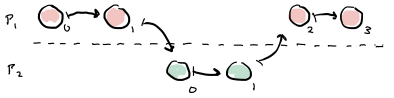
\includegraphics[scale=0.7]{images/yieldcoproduct.png}
\caption{Illustration of the yielding coproduct process. It is capable of switching between the two processes, as illustrated by the calls to v1 and v2.}
\end{figure}

%
With a combinator such as this one could you model e.g a two player game.
%
The processes would be the players and the combined process allows each to take turns making their next move.
%
In section \ref{subsec:policycombinators} we discuss how a policy for such a process is something of a game leader.
%

%
A unit to the yielding coproduct combinator is the same one as that for the regular coproduct combinator.
%
If the state space is not inhabited, the process could never progress as we will not be able to call the step function.
%
Further more, we would not be able to give a definition for a function \ensuremath{\Conid{S₁}\;\to \;\Conid{S₂}}.
%

%-----------------------------------------------------------------------
\subsubsection{Interleaving processes}
\label{subsubsec:interleavingseqdecproc}
%
The next combinator we introduce is one that interleaves processes.
%
The state of such a process holds components of both prior states, but takes turns applying the step function to each of them.
%
This behaviour could be similar to that of a game, where two players take turns making their next move.
%
However, the users do not know what moves the other player has made, and can therefore not make particularly smart moves.
%
In section \ref{subsec:policycombinators} it is reasoned that writing new policies for a process like this will be a policy that does know what move the other 'player' has made.
%

%
Similar to the product combinator the new state needs to hold components of both prior states.
%
It should apply the step function to them one at a time, alternating between the two.
%
In order to know which components turn it is to advance we extend the product to also hold an index.
%
\begin{hscode}\SaveRestoreHook
\column{B}{@{}>{\hspre}l<{\hspost}@{}}%
\column{E}{@{}>{\hspre}l<{\hspost}@{}}%
\>[B]{}\unopun{\mathop{⇄_{\!S}}}\;\mathbin{:}\;\Conid{Set}\;\Varid{→}\;\Conid{Set}\;\Varid{→}\;\Conid{Set}{}\<[E]%
\\
\>[B]{}\Conid{S₁}\;\mathop{⇄_{\!S}}\;\Conid{S₂}\;\mathrel{=}\;\Conid{Fin}\;\Varid{2}\;\Varid{×}\;\Conid{S₁}\;\Varid{×}\;\Conid{S₂}{}\<[E]%
\ColumnHook
\end{hscode}\resethooks
%
The control space for the interleaved process is the sum of the two prior control spaces.
%
If the value of the first component is zero, we select the first control.
%
If the value is one, we select the second control.
%
\begin{hscode}\SaveRestoreHook
\column{B}{@{}>{\hspre}l<{\hspost}@{}}%
\column{7}{@{}>{\hspre}l<{\hspost}@{}}%
\column{10}{@{}>{\hspre}l<{\hspost}@{}}%
\column{30}{@{}>{\hspre}l<{\hspost}@{}}%
\column{E}{@{}>{\hspre}l<{\hspost}@{}}%
\>[B]{}\Varid{one}\;\mathbin{:}\;\Conid{Fin}\;\Varid{2}{}\<[E]%
\\
\>[B]{}\Varid{one}\;\mathrel{=}\;\Varid{suc}\;\Varid{zero}{}\<[E]%
\\[\blanklineskip]%
\>[B]{}\unopun{\mathop{⇄_C}}\;{}\<[7]%
\>[7]{}\mathbin{:}\;{}\<[10]%
\>[10]{}\{\mskip1.5mu \Conid{S₁}\;\Conid{S₂}\;\mathbin{:}\;\Conid{Set}\mskip1.5mu\}\;{}\<[E]%
\\
\>[7]{}\Varid{→}\;{}\<[10]%
\>[10]{}\Conid{Con}\;\Conid{S₁}\;\Varid{→}\;\Conid{Con}\;\Conid{S₂}\;\Varid{→}\;\Conid{Con}\;(\Conid{S₁}\;\mathop{⇄_{\!S}}\;\Conid{S₂}){}\<[E]%
\\
\>[B]{}(\Conid{C₁}\;\mathop{⇄_C}\;\Conid{C₂})\;(\Varid{zero}\;\Varid{,}\;\Varid{s₁}\;\Varid{,}\;\Varid{s₂})\;{}\<[30]%
\>[30]{}\mathrel{=}\;\Conid{C₁}\;\Varid{s₁}{}\<[E]%
\\
\>[B]{}(\Conid{C₁}\;\mathop{⇄_C}\;\Conid{C₂})\;(\Varid{one}\;\Varid{,}\;\Varid{s₁}\;\Varid{,}\;\Varid{s₂})\;{}\<[30]%
\>[30]{}\mathrel{=}\;\Conid{C₂}\;\Varid{s₂}{}\<[E]%
\ColumnHook
\end{hscode}\resethooks
%
Defining a new step function in terms of the two previous ones is done by pattern matching on the state.
%
Specifically we are interested in the first component, the index.
%
If the index is zero we apply the first step function to the second component of the state, leave the last component unchanged and increment the index by one.
%
Similarly if the index is zero we apply the second step function to the last component, leave the second one unchanged and decrement the index by one.
%
\begin{hscode}\SaveRestoreHook
\column{B}{@{}>{\hspre}l<{\hspost}@{}}%
\column{8}{@{}>{\hspre}l<{\hspost}@{}}%
\column{11}{@{}>{\hspre}l<{\hspost}@{}}%
\column{35}{@{}>{\hspre}l<{\hspost}@{}}%
\column{40}{@{}>{\hspre}l<{\hspost}@{}}%
\column{E}{@{}>{\hspre}l<{\hspost}@{}}%
\>[B]{}\unopun{\mathop{⇄_{\text{sf}}}}\;{}\<[8]%
\>[8]{}\mathbin{:}\;{}\<[11]%
\>[11]{}\{\mskip1.5mu \Conid{S₁}\;\Conid{S₂}\;\mathbin{:}\;\Conid{Set}\mskip1.5mu\}\;{}\<[E]%
\\
\>[8]{}\Varid{→}\;{}\<[11]%
\>[11]{}\{\mskip1.5mu \Conid{C₁}\;\mathbin{:}\;\Conid{Con}\;\Conid{S₁}\mskip1.5mu\}\;\Varid{→}\;\{\mskip1.5mu \Conid{C₂}\;\mathbin{:}\;\Conid{Con}\;\Conid{S₂}\mskip1.5mu\}\;{}\<[E]%
\\
\>[8]{}\Varid{→}\;{}\<[11]%
\>[11]{}\Conid{Step}\;\Conid{S₁}\;\Conid{C₁}\;\Varid{→}\;\Conid{Step}\;\Conid{S₂}\;\Conid{C₂}\;{}\<[E]%
\\
\>[8]{}\Varid{→}\;{}\<[11]%
\>[11]{}\Conid{Step}\;(\Conid{S₁}\;\mathop{⇄_{\!S}}\;\Conid{S₂})\;(\Conid{C₁}\;\mathop{⇄_C}\;\Conid{C₂}){}\<[E]%
\\
\>[B]{}(\Varid{sf₁}\;\mathop{⇄_{\text{sf}}}\;\Varid{sf₂})\;(\Varid{zero}\;\Varid{,}\;\Varid{s₁}\;\Varid{,}\;\Varid{s₂})\;\Varid{c}\;{}\<[35]%
\>[35]{}\mathrel{=}\;(\Varid{one}\;\Varid{,}\;\Varid{sf₁}\;\Varid{s₁}\;\Varid{c}\;\Varid{,}\;\Varid{s₂}){}\<[E]%
\\
\>[B]{}(\Varid{sf₁}\;\mathop{⇄_{\text{sf}}}\;\Varid{sf₂})\;(\Varid{suc}\;\Varid{zero}\;\Varid{,}\;\Varid{s₁}\;\Varid{,}\;\Varid{s₂})\;\Varid{c}\;{}\<[40]%
\>[40]{}\mathrel{=}\;(\Varid{zero}\;\Varid{,}\;\Varid{s₁}\;\Varid{,}\;\Varid{sf₂}\;\Varid{s₂}\;\Varid{c}){}\<[E]%
\\
\>[B]{}(\Varid{sf₁}\;\mathop{⇄_{\text{sf}}}\;\Varid{sf₂})\;(\Varid{suc}\;(\Varid{suc}\;())\;\Varid{,}\;\anonymous \;\Varid{,}\;\anonymous ){}\<[E]%
\ColumnHook
\end{hscode}\resethooks
%
Combining two processes to capture this interleaved behaviour is once again simply done by combining the components componentwise.
%
\begin{hscode}\SaveRestoreHook
\column{B}{@{}>{\hspre}l<{\hspost}@{}}%
\column{3}{@{}>{\hspre}l<{\hspost}@{}}%
\column{E}{@{}>{\hspre}l<{\hspost}@{}}%
\>[B]{}\unopun{\mathop{⇄_{\text{SDP}}}}\;\mathbin{:}\;\Conid{SDProc}\;\Varid{→}\;\Conid{SDProc}\;\Varid{→}\;\Conid{SDProc}{}\<[E]%
\\
\>[B]{}\Conid{SDP}\;\Conid{S₁}\;\Conid{C₁}\;\Varid{sf₁}\;\mathop{⇄_{\text{SDP}}}\;\Conid{SDP}\;\Conid{S₂}\;\Conid{C₂}\;\Varid{sf₂}\;{}\<[E]%
\\
\>[B]{}\hsindent{3}{}\<[3]%
\>[3]{}\mathrel{=}\;\Conid{SDP}\;(\Conid{S₁}\;\mathop{⇄_{\!S}}\;\Conid{S₂})\;(\Conid{C₁}\;\mathop{⇄_C}\;\Conid{C₂})\;(\Varid{sf₁}\;\mathop{⇄_{\text{sf}}}\;\Varid{sf₂}){}\<[E]%
\ColumnHook
\end{hscode}\resethooks
%
The final process behaves as illustrated in figure \ref{images:interleave}.
%

\begin{figure}
\centering
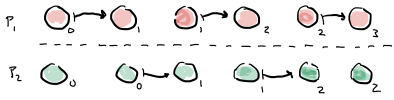
\includegraphics[scale=0.7]{images/interleave.png}
\caption{Illustration of two interleaved process. We want to emphasise that the state holds components of both prior states, but chooses to advance only one. The policy that chooses what control to use can however inspect both components.}
\label{images:interleave}
\end{figure}

%
Defining a unit for the interleaved process is not possible.
%
Where the initial process would advance e.g five steps, the interleaved process would need ten steps to take that component to the same state.
%
We can not give a generic process that when interleaved with another process acts as a unit.

The way we define the interleaved combinator might not be optimal.
%
Combining more than two processes will produce potentially unexpected behaviour.
%
If we combine three processes using this combinator the resulting system would be one where one of the processes advance half the time, and the other two only a quarter of the time each.
%
\begin{figure*}[htbp]
  \begin{subfigure}[b]{.8\textwidth}
    \centering
    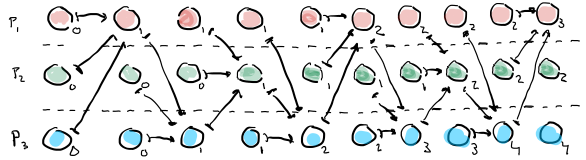
\includegraphics[scale=0.8]{images/badinterleave2.png}
    \caption{If we interleave two processes and then interleave the resulting process with a third we get a situation like this. They are not properly interleaved.}
    \label{images:badinterleave}
  \end{subfigure}
  \begin{subfigure}[b]{.8\textwidth}
    \centering
    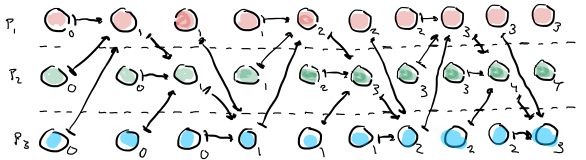
\includegraphics[scale=0.8]{images/wantedinterleave2.png}
    \caption{This is the interleaved behaviour we might expect for three processes. A round robin behaviour that gives the processes equally many turns.}
    \label{images:wantedinterleave}
  \end{subfigure}
  \caption{Illustrations of why the interleaved combinator might not behave as one would expect. Again the two incoming arrows illustrate that the policy that selects the control has access to all components and can base the choice of control on them.}
  \label{images:badvsgoodinterleave}
\end{figure*}

%
This does not necessarily mean that the combinator described in Figure \ref{images:badvsgoodinterleave}  is wrong, but rather that there is another combinator we could implement that would have this other behaviour.
%
%------------------------------------------------------------------------------
% -*- latex -*-
\subsection{Time dependent processes}
\label{subsec:timedependentcase}

%
Imagine a process where the state space can vary over time.
%
If we consider the example with the one dimensional coordinate system, if the process is time dependent it could disallow some states at certain points in time.
%
Below we illustrate how this is defined in Agda.
%
\begin{hscode}\SaveRestoreHook
\column{B}{@{}>{\hspre}l<{\hspost}@{}}%
\column{3}{@{}>{\hspre}l<{\hspost}@{}}%
\column{5}{@{}>{\hspre}l<{\hspost}@{}}%
\column{14}{@{}>{\hspre}l<{\hspost}@{}}%
\column{E}{@{}>{\hspre}l<{\hspost}@{}}%
\>[B]{}\Conid{ConT}\;\mathbin{:}\;(\Conid{ℕ}\;\to \;\Conid{Set})\;\Varid{→}\;\Conid{Set₁}{}\<[E]%
\\
\>[B]{}\Conid{ConT}\;\Conid{S}\;\mathrel{=}\;(\Varid{t}\;\mathbin{:}\;\Conid{ℕ})\;\to \;\Conid{S}\;\Varid{t}\;\Varid{→}\;\Conid{Set}{}\<[E]%
\\[\blanklineskip]%
\>[B]{}\Conid{StepT}\;\mathbin{:}\;(\Conid{S}\;\mathbin{:}\;\Conid{ℕ}\;\to \;\Conid{Set})\;\to \;\Conid{ConT}\;\Conid{S}\;\to \;\Conid{Set}{}\<[E]%
\\
\>[B]{}\Conid{StepT}\;\Conid{S}\;\Conid{C}\;\mathrel{=}\;(\Varid{t}\;\mathbin{:}\;\Conid{ℕ})\;\to \;(\Varid{s}\;\mathbin{:}\;\Conid{S}\;\Varid{t})\;\to \;\Conid{C}\;\Varid{t}\;\Varid{s}\;\to \;\Conid{S}\;(\Varid{suc}\;\Varid{t}){}\<[E]%
\\[\blanklineskip]%
\>[B]{}\mathbf{record}\;\Conid{SDProcT}\;\mathbin{:}\;\Conid{Set₁}\;\mathbf{where}{}\<[E]%
\\
\>[B]{}\hsindent{3}{}\<[3]%
\>[3]{}\Varid{constructor}\;\Conid{SDPT}{}\<[E]%
\\
\>[B]{}\hsindent{3}{}\<[3]%
\>[3]{}\mathbf{field}{}\<[E]%
\\
\>[3]{}\hsindent{2}{}\<[5]%
\>[5]{}\Conid{State}\;{}\<[14]%
\>[14]{}\mathbin{:}\;\Conid{ℕ}\;\Varid{→}\;\Conid{Set}{}\<[E]%
\\
\>[3]{}\hsindent{2}{}\<[5]%
\>[5]{}\Conid{Control}\;{}\<[14]%
\>[14]{}\mathbin{:}\;\Conid{ConT}\;\Conid{State}{}\<[E]%
\\
\>[3]{}\hsindent{2}{}\<[5]%
\>[5]{}\Varid{step}\;{}\<[14]%
\>[14]{}\mathbin{:}\;\Conid{StepT}\;\Conid{State}\;\Conid{Control}{}\<[E]%
\ColumnHook
\end{hscode}\resethooks
%
The state is now dependent on a parameter \ensuremath{\Varid{t}\;\mathbin{:}\;\Conid{ℕ}}, which allows the state to take on alternate forms.
%
In section \ref{subsubsec:timedependentexample} we illustrate what this means.
%

%
A time independent process can be embedded as a time dependent process.
%
The embedding is a process that disregards the time parameter.
%
\begin{hscode}\SaveRestoreHook
\column{B}{@{}>{\hspre}l<{\hspost}@{}}%
\column{3}{@{}>{\hspre}l<{\hspost}@{}}%
\column{E}{@{}>{\hspre}l<{\hspost}@{}}%
\>[B]{}\Varid{embed}\;\mathbin{:}\;\Conid{SDProc}\;\Varid{→}\;\Conid{SDProcT}{}\<[E]%
\\
\>[B]{}\Varid{embed}\;(\Conid{SDP}\;\Conid{S}\;\Conid{C}\;\Varid{sf})\;{}\<[E]%
\\
\>[B]{}\hsindent{3}{}\<[3]%
\>[3]{}\mathrel{=}\;\Conid{SDPT}\;(\lambda\;\anonymous \;\Varid{→}\;\Conid{S})\;(\lambda\;\anonymous \;\Varid{→}\;\Conid{C})\;(\lambda\;\anonymous \;\Varid{→}\;\Varid{sf}){}\<[E]%
\ColumnHook
\end{hscode}\resethooks

\subsection{A discussion on the \ensuremath{\Conid{Fin}} type}
\label{subsec:fintype}
%
Before we move on to an example of a time dependent process, we need to briefly present the \ensuremath{\Conid{Fin}} type and its properties.
%
The \ensuremath{\Conid{Fin}\;\Varid{n}} type (for any natural number \ensuremath{\Varid{n}}) has exactly \ensuremath{\Varid{n}} elements.
%
\begin{hscode}\SaveRestoreHook
\column{B}{@{}>{\hspre}l<{\hspost}@{}}%
\column{3}{@{}>{\hspre}l<{\hspost}@{}}%
\column{5}{@{}>{\hspre}l<{\hspost}@{}}%
\column{11}{@{}>{\hspre}l<{\hspost}@{}}%
\column{34}{@{}>{\hspre}l<{\hspost}@{}}%
\column{E}{@{}>{\hspre}l<{\hspost}@{}}%
\>[3]{}\mathbf{data}\;\Conid{Fin}\;\mathbin{:}\;\Conid{ℕ}\;\Varid{→}\;\Conid{Set}\;\mathbf{where}{}\<[E]%
\\
\>[3]{}\hsindent{2}{}\<[5]%
\>[5]{}\Varid{zero}\;{}\<[11]%
\>[11]{}\mathbin{:}\;\{\mskip1.5mu \Varid{n}\;\mathbin{:}\;\Conid{ℕ}\mskip1.5mu\}\;{}\<[34]%
\>[34]{}\Varid{→}\;\Conid{Fin}\;(\Varid{suc}\;\Varid{n}){}\<[E]%
\\
\>[3]{}\hsindent{2}{}\<[5]%
\>[5]{}\Varid{suc}\;{}\<[11]%
\>[11]{}\mathbin{:}\;\{\mskip1.5mu \Varid{n}\;\mathbin{:}\;\Conid{ℕ}\mskip1.5mu\}\;(\Varid{i}\;\mathbin{:}\;\Conid{Fin}\;\Varid{n})\;{}\<[34]%
\>[34]{}\Varid{→}\;\Conid{Fin}\;(\Varid{suc}\;\Varid{n}){}\<[E]%
\ColumnHook
\end{hscode}\resethooks
%
From this definition we see that \ensuremath{\Varid{zero}} is an element of \ensuremath{\Conid{Fin}\;\Varid{n}} for any \ensuremath{\Varid{n}\;\Varid{>}\;\Varid{zero}}.
%
The constructor \ensuremath{\Varid{suc}} takes an element of type \ensuremath{\Conid{Fin}\;\Varid{n}} and returns an element of type \ensuremath{\Conid{Fin}\;(\Varid{suc}\;\Varid{n})}.
%
We illustrate the type for a couple of different n's in figure \ref{images:finn}.
%
\begin{figure}
\centering
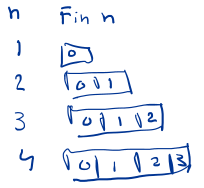
\includegraphics[scale=0.7]{images/finn.png}
\caption{An illustration of the \ensuremath{\Conid{Fin}\;\Varid{n}} type. We emphasise that there are exactly \ensuremath{\Varid{n}} inhabitants of \ensuremath{\Conid{Fin}\;\Varid{n}}.}
\label{images:finn}
\end{figure}

\begin{figure*}[htbp]
  \begin{subfigure}[b]{.20\textwidth}
    \hbox{\hspace{-0.5em} 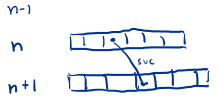
\includegraphics[scale=0.75]{images/suc.png}}
    \caption{}
    \label{images:suc}
  \end{subfigure}
  \begin{subfigure}[b]{.20\textwidth}
    \centering
    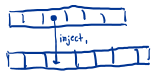
\includegraphics[scale=0.75]{images/inject.png}
    \caption{}
    \label{images:inject}
  \end{subfigure}
  \begin{subfigure}[b]{.20\textwidth}
    \centering
    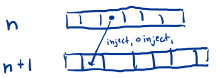
\includegraphics[scale=0.75]{images/injectinject.png}
    \caption{}
    \label{images:injectinject}
  \end{subfigure}
  \begin{subfigure}[b]{.20\textwidth}
    \centering
    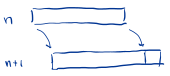
\includegraphics[scale=0.75]{images/embed.png}
    \caption{}
    \label{images:embed}
  \end{subfigure}

  \caption{Illustrations of how to embed elements of type \ensuremath{\Conid{Fin}\;\Varid{n}} in the sucessor type \ensuremath{\Conid{Fin}\;(\Varid{suc}\;\Varid{n})}.}
  \label{images:fin}
\end{figure*}

%
We illustrate what the \ensuremath{\Varid{suc}} constructor does in figure \ref{images:suc}.
%
It takes an element of type \ensuremath{\Conid{Fin}\;\Varid{n}}, and returns the sucessor element of type \ensuremath{\Conid{Fin}\;(\Varid{suc}\;\Varid{n})}.
%

%
What if we want an element of the sucessor type without using the suc constructor?
%
We might wish to simply 'promote' the type of an element.
%
In figure \ref{images:embed} it becomes clear that all elements of type \ensuremath{\Conid{Fin}\;\Varid{n}} are also elements of \ensuremath{\Conid{Fin}\;(\Varid{suc}\;\Varid{n})}.
%
To do this promoting we use the function inject₁, which is illustrated in figure \ref{images:inject}.
%
\begin{hscode}\SaveRestoreHook
\column{B}{@{}>{\hspre}l<{\hspost}@{}}%
\column{3}{@{}>{\hspre}l<{\hspost}@{}}%
\column{20}{@{}>{\hspre}l<{\hspost}@{}}%
\column{E}{@{}>{\hspre}l<{\hspost}@{}}%
\>[3]{}\Varid{inject₁}\;\mathbin{:}\;\Varid{∀}\;\{\mskip1.5mu \Varid{m}\mskip1.5mu\}\;\Varid{→}\;\Conid{Fin}\;\Varid{m}\;\Varid{→}\;\Conid{Fin}\;(\Varid{suc}\;\Varid{m}){}\<[E]%
\\
\>[3]{}\Varid{inject₁}\;\Varid{zero}\;{}\<[20]%
\>[20]{}\mathrel{=}\;\Varid{zero}{}\<[E]%
\\
\>[3]{}\Varid{inject₁}\;(\Varid{suc}\;\Varid{i})\;{}\<[20]%
\>[20]{}\mathrel{=}\;\Varid{suc}\;(\Varid{inject₁}\;\Varid{i}){}\<[E]%
\ColumnHook
\end{hscode}\resethooks
%

Now, what if we find ourselves in a situation where we have an element of type \ensuremath{\Conid{Fin}\;(\Varid{suc}\;\Varid{n})}, and we want to return its predecessor, but of the sucessor type \emph{Fin (suc (suc n))}?
%
What we want to do is given an element \ensuremath{\Varid{suc}\;\Varid{x}}, return \ensuremath{\Varid{x}}.
%
We can't do this as is since the element \ensuremath{\Varid{suc}\;\Varid{x}} is of type \ensuremath{\Conid{Fin}\;(\Varid{suc}\;\Varid{n})}, the element \ensuremath{\Varid{x}} is of type \ensuremath{\Conid{Fin}\;\Varid{n}}.
%
To get the proper type we need to invoke \ensuremath{\Varid{inject₁}} twice, which is illustrated in figure \ref{images:injectinject}.

\subsubsection{Time dependent example}
\label{subsubsec:timedependentexample}
%
Looking back at the time independent example, we reflect on the choice of state.
%
The natural numbers seemed, and were, a reasonable choice.
%
With the time dependent process at our disposal however we notice a source of ineffectiveness.
%

%
We consider the case where the process is always evaluated with \ensuremath{\Varid{zero}} as the initial state.
%
After 1 step we could either have stayed or we went right, meaning the state is now \ensuremath{\Varid{zero}} or \ensuremath{\Varid{suc}\;\Varid{zero}}.
%
After 2 steps we could have gone left, stayed or gone right.
%
In figure \ref{fig:edgecasefin} this edge case is illustrated, and we note that the number of possible states after n steps is \ensuremath{\Varid{n+1}}.
%
\begin{figure}[H]
  \centering
  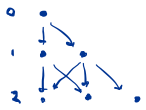
\includegraphics[scale=0.75]{images/edgecasefin}
  \caption{In the edge case the state space grows slower, as we initially can not decrement the state.}
  \label{fig:edgecasefin}
\end{figure}
%
If we consider the example from earlier but restrict it to starting in state zero, we could define this process as follows.
%
\begin{hscode}\SaveRestoreHook
\column{B}{@{}>{\hspre}l<{\hspost}@{}}%
\column{E}{@{}>{\hspre}l<{\hspost}@{}}%
\>[B]{}\Varid{1\!d\text{-}state}\;\mathbin{:}\;\Conid{ℕ}\;\Varid{→}\;\Conid{Set}{}\<[E]%
\\
\>[B]{}\Varid{1\!d\text{-}state}\;\Varid{n}\;\mathrel{=}\;\Conid{Fin}\;(\Varid{suc}\;\Varid{n}){}\<[E]%
\ColumnHook
\end{hscode}\resethooks
%
The Agda type \ensuremath{\Conid{Fin}\;\Varid{n}} is a type with at most \ensuremath{\Varid{n}} elements.
%
Using this type gives us a more precise definition of what the possible states are.
%

%
The controls are identical to those in the time independent case.
\begin{hscode}\SaveRestoreHook
\column{B}{@{}>{\hspre}l<{\hspost}@{}}%
\column{25}{@{}>{\hspre}l<{\hspost}@{}}%
\column{E}{@{}>{\hspre}l<{\hspost}@{}}%
\>[B]{}\Varid{1d\text{-}control}\;\mathbin{:}\;(\Varid{n}\;\mathbin{:}\;\Conid{ℕ})\;\Varid{→}\;\Varid{1\!d\text{-}state}\;\Varid{n}\;\Varid{→}\;\Conid{Set}{}\<[E]%
\\
\>[B]{}\Varid{1d\text{-}control}\;\Varid{n}\;\Varid{zero}\;{}\<[25]%
\>[25]{}\mathrel{=}\;\Conid{ZAction}{}\<[E]%
\\
\>[B]{}\Varid{1d\text{-}control}\;\Varid{n}\;(\Varid{suc}\;\Varid{x})\;{}\<[25]%
\>[25]{}\mathrel{=}\;\Conid{SAction}{}\<[E]%
\ColumnHook
\end{hscode}\resethooks

%
The step function says the same thing as in the previous example, but it says it a little differently.
%
If the state is zero there is only two available controls, and we update the state like we did previously.
%
However, if the state is greater than \ensuremath{\Varid{zero}} we need to change the types as described in section \ref{subsec:fintype}.
%
For the left control the result has to be injected twice, and for the stay control it has to be injected once.
%
\begin{hscode}\SaveRestoreHook
\column{B}{@{}>{\hspre}l<{\hspost}@{}}%
\column{12}{@{}>{\hspre}l<{\hspost}@{}}%
\column{15}{@{}>{\hspre}l<{\hspost}@{}}%
\column{22}{@{}>{\hspre}l<{\hspost}@{}}%
\column{26}{@{}>{\hspre}l<{\hspost}@{}}%
\column{41}{@{}>{\hspre}l<{\hspost}@{}}%
\column{E}{@{}>{\hspre}l<{\hspost}@{}}%
\>[B]{}\Varid{1d\text{-}step}\;{}\<[12]%
\>[12]{}\mathbin{:}\;{}\<[15]%
\>[15]{}(\Varid{n}\;\mathbin{:}\;\Conid{ℕ})\;\Varid{→}\;(\Varid{x}\;\mathbin{:}\;\Varid{1\!d\text{-}state}\;\Varid{n})\;{}\<[E]%
\\
\>[12]{}\Varid{→}\;{}\<[15]%
\>[15]{}(\Varid{y}\;\mathbin{:}\;\Varid{1d\text{-}control}\;\Varid{n}\;\Varid{x})\;\Varid{→}\;{}\<[41]%
\>[41]{}\Varid{1\!d\text{-}state}\;(\Varid{suc}\;\Varid{n}){}\<[E]%
\\
\>[B]{}\Varid{1d\text{-}step}\;\Varid{n}\;\Varid{zero}\;{}\<[22]%
\>[22]{}\Conid{ZS}\;{}\<[26]%
\>[26]{}\mathrel{=}\;\Varid{zero}{}\<[E]%
\\
\>[B]{}\Varid{1d\text{-}step}\;\Varid{n}\;\Varid{zero}\;{}\<[22]%
\>[22]{}\Conid{ZR}\;{}\<[26]%
\>[26]{}\mathrel{=}\;\Varid{suc}\;\Varid{zero}{}\<[E]%
\\
\>[B]{}\Varid{1d\text{-}step}\;\Varid{n}\;(\Varid{suc}\;\Varid{x})\;{}\<[22]%
\>[22]{}\Conid{SL}\;{}\<[26]%
\>[26]{}\mathrel{=}\;\Varid{inject₁}\;(\Varid{inject₁}\;\Varid{x}){}\<[E]%
\\
\>[B]{}\Varid{1d\text{-}step}\;\Varid{n}\;(\Varid{suc}\;\Varid{x})\;{}\<[22]%
\>[22]{}\Conid{SS}\;{}\<[26]%
\>[26]{}\mathrel{=}\;\Varid{inject₁}\;(\Varid{suc}\;\Varid{x}){}\<[E]%
\\
\>[B]{}\Varid{1d\text{-}step}\;\Varid{n}\;(\Varid{suc}\;\Varid{x})\;{}\<[22]%
\>[22]{}\Conid{SR}\;{}\<[26]%
\>[26]{}\mathrel{=}\;\Varid{suc}\;(\Varid{suc}\;\Varid{x}){}\<[E]%
\ColumnHook
\end{hscode}\resethooks
%
Now the entire system has been defined and we can package it as a \ensuremath{\Conid{SDProcT}}.
%
\begin{hscode}\SaveRestoreHook
\column{B}{@{}>{\hspre}l<{\hspost}@{}}%
\column{E}{@{}>{\hspre}l<{\hspost}@{}}%
\>[B]{}\Varid{finsystem}\;\mathbin{:}\;\Conid{SDProcT}{}\<[E]%
\\
\>[B]{}\Varid{finsystem}\;\mathrel{=}\;\Conid{SDPT}\;\Varid{1\!d\text{-}state}\;\Varid{1d\text{-}control}\;\Varid{1d\text{-}step}{}\<[E]%
\ColumnHook
\end{hscode}\resethooks
%------------------------------------------------------------------------------
% -*- Latex -*-
\subsection{Combinators for the Time Dependent Case}
\label{subsec:combinatorstime}
%
Before we move on we want to highlight that the state now is dependent on the natural numbers.
%
The controls of these time dependent processes are time dependent themselves.
%
We capture this reasoning in the definition of \ensuremath{\Conid{Con'}}.
%
\begin{hscode}\SaveRestoreHook
\column{B}{@{}>{\hspre}l<{\hspost}@{}}%
\column{E}{@{}>{\hspre}l<{\hspost}@{}}%
\>[B]{}\Conid{Con'}\;\mathbin{:}\;\Conid{Con}\;\Conid{ℕ}\;\Varid{→}\;\Conid{Set₁}{}\<[E]%
\\
\>[B]{}\Conid{Con'}\;\Conid{S}\;\mathrel{=}\;(\Varid{t}\;\mathbin{:}\;\Conid{ℕ})\;\Varid{→}\;\Conid{Con}\;(\Conid{S}\;\Varid{t}){}\<[E]%
\ColumnHook
\end{hscode}\resethooks
%
Now on to the product combinator for the time dependent case.
%
To combine two states that are time dependent we compute a new time dependent state that is the product of applying the prior states to the time.
%
\begin{hscode}\SaveRestoreHook
\column{B}{@{}>{\hspre}l<{\hspost}@{}}%
\column{E}{@{}>{\hspre}l<{\hspost}@{}}%
\>[B]{}\unopun{×_{\!\Varid{S}}}\;\mathbin{:}\;(\Conid{S₁}\;\Conid{S₂}\;\mathbin{:}\;\Conid{Con}\;\Conid{ℕ})\;\Varid{→}\;\Conid{Con}\;\Conid{ℕ}{}\<[E]%
\\
\>[B]{}\Varid{s₁}\;×_{\!\Varid{S}}\;\Varid{s₂}\;\mathrel{=}\;\lambda\;\Varid{t}\;\Varid{→}\;\Varid{s₁}\;\Varid{t}\;\Varid{×}\;\Varid{s₂}\;\Varid{t}{}\<[E]%
\ColumnHook
\end{hscode}\resethooks
%
The product combinator for two controls should produce a new \ensuremath{\Conid{Con'}} on \ensuremath{\Conid{S₁}\;×_{\!\Varid{S}}\;\Conid{S₂}} defined in terms of two controls \ensuremath{\Conid{Con'}\;\Conid{S₁}} and \ensuremath{\Conid{Con'}\;\Conid{S₂}}.
%
The defining equation is similar to the time independent case, but the extra parameter time is given as the first argument.
%
\begin{hscode}\SaveRestoreHook
\column{B}{@{}>{\hspre}l<{\hspost}@{}}%
\column{7}{@{}>{\hspre}l<{\hspost}@{}}%
\column{11}{@{}>{\hspre}l<{\hspost}@{}}%
\column{13}{@{}>{\hspre}l<{\hspost}@{}}%
\column{33}{@{}>{\hspre}l<{\hspost}@{}}%
\column{36}{@{}>{\hspre}l<{\hspost}@{}}%
\column{E}{@{}>{\hspre}l<{\hspost}@{}}%
\>[B]{}\unopun{\mathop{×_{\!\Varid{C}}}}\;{}\<[7]%
\>[7]{}\mathbin{:}\;{}\<[11]%
\>[11]{}\{\mskip1.5mu \Conid{S₁}\;\Conid{S₂}\;\mathbin{:}\;\Conid{Con}\;\Conid{ℕ}\mskip1.5mu\}\;{}\<[E]%
\\
\>[7]{}\Varid{→}\;{}\<[13]%
\>[13]{}\Conid{Con'}\;\Conid{S₁}\;\Varid{→}\;\Conid{Con'}\;\Conid{S₂}\;{}\<[33]%
\>[33]{}\Varid{→}\;{}\<[36]%
\>[36]{}\Conid{Con'}\;(\Conid{S₁}\;×_{\!\Varid{S}}\;\Conid{S₂}){}\<[E]%
\\
\>[B]{}(\Conid{C₁}\;\mathop{×_{\!\Varid{C}}}\;\Conid{C₂})\;\Varid{time}\;(\Varid{s₁}\;\Varid{,}\;\Varid{s₂})\;\mathrel{=}\;\Conid{C₁}\;\Varid{time}\;\Varid{s₁}\;\Varid{×}\;\Conid{C₂}\;\Varid{time}\;\Varid{s₂}{}\<[E]%
\ColumnHook
\end{hscode}\resethooks
%
Again we capture the type of the step function in a type \ensuremath{\Conid{Step}}.
%
\ensuremath{\Conid{Step}} accepts a state and a control and returns a type.
%
The type is that of the step function for time dependent processes.
%
\begin{hscode}\SaveRestoreHook
\column{B}{@{}>{\hspre}l<{\hspost}@{}}%
\column{E}{@{}>{\hspre}l<{\hspost}@{}}%
\>[B]{}\Conid{Step}\;\mathbin{:}\;(\Conid{S}\;\mathbin{:}\;\Conid{Con}\;\Conid{ℕ})\;\to \;\Conid{Con'}\;\Conid{S}\;\to \;\Conid{Set}{}\<[E]%
\\
\>[B]{}\Conid{Step}\;\Conid{S}\;\Conid{C}\;\mathrel{=}\;(\Varid{t}\;\mathbin{:}\;\Conid{ℕ})\;\Varid{→}\;(\Varid{s}\;\mathbin{:}\;\Conid{S}\;\Varid{t})\;\to \;\Conid{C}\;\Varid{t}\;\Varid{s}\;\to \;\Conid{S}\;(\Varid{suc}\;\Varid{t}){}\<[E]%
\ColumnHook
\end{hscode}\resethooks
%
Combining two such step functions is similar to the time independent case.
%
The only different is that we have an extra parameter \ensuremath{\Varid{time}}, and we must apply the step functions to this \ensuremath{\Varid{time}} parameters.
%
\begin{hscode}\SaveRestoreHook
\column{B}{@{}>{\hspre}l<{\hspost}@{}}%
\column{3}{@{}>{\hspre}l<{\hspost}@{}}%
\column{6}{@{}>{\hspre}l<{\hspost}@{}}%
\column{8}{@{}>{\hspre}l<{\hspost}@{}}%
\column{11}{@{}>{\hspre}l<{\hspost}@{}}%
\column{E}{@{}>{\hspre}l<{\hspost}@{}}%
\>[B]{}\unopun{×_{\!\Varid{sf}}}\;{}\<[8]%
\>[8]{}\mathbin{:}\;{}\<[11]%
\>[11]{}\{\mskip1.5mu \Conid{S₁}\;\Conid{S₂}\;\mathbin{:}\;\Conid{Con}\;\Conid{ℕ}\mskip1.5mu\}\;{}\<[E]%
\\
\>[8]{}\Varid{→}\;{}\<[11]%
\>[11]{}\{\mskip1.5mu \Conid{C₁}\;\mathbin{:}\;\Conid{Con'}\;\Conid{S₁}\mskip1.5mu\}\;\Varid{→}\;\{\mskip1.5mu \Conid{C₂}\;\mathbin{:}\;\Conid{Con'}\;\Conid{S₂}\mskip1.5mu\}\;{}\<[E]%
\\
\>[8]{}\Varid{→}\;{}\<[11]%
\>[11]{}\Conid{Step}\;\Conid{S₁}\;\Conid{C₁}\;\Varid{→}\;\Conid{Step}\;\Conid{S₂}\;\Conid{C₂}\;{}\<[E]%
\\
\>[8]{}\Varid{→}\;{}\<[11]%
\>[11]{}\Conid{Step}\;(\Conid{S₁}\;×_{\!\Varid{S}}\;\Conid{S₂})\;(\Conid{C₁}\;\mathop{×_{\!\Varid{C}}}\;\Conid{C₂}){}\<[E]%
\\
\>[B]{}(\Varid{sf₁}\;×_{\!\Varid{sf}}\;\Varid{sf₂})\;\Varid{time}\;\Varid{state}\;\Varid{control}\;{}\<[E]%
\\
\>[B]{}\hsindent{3}{}\<[3]%
\>[3]{}\mathrel{=}\;{}\<[6]%
\>[6]{}\Varid{sf₁}\;\Varid{time}\;(\Varid{proj₁}\;\Varid{state})\;(\Varid{proj₁}\;\Varid{control})\;\Varid{,}\;{}\<[E]%
\\
\>[6]{}\Varid{sf₂}\;\Varid{time}\;(\Varid{proj₂}\;\Varid{state})\;(\Varid{proj₂}\;\Varid{control}){}\<[E]%
\ColumnHook
\end{hscode}\resethooks
%
Finally, combining two time dependent sequential decision processes is done by applying the combinators componentwise.
%
\begin{hscode}\SaveRestoreHook
\column{B}{@{}>{\hspre}l<{\hspost}@{}}%
\column{3}{@{}>{\hspre}l<{\hspost}@{}}%
\column{E}{@{}>{\hspre}l<{\hspost}@{}}%
\>[B]{}\unopun{×_{\!\Varid{SDP}}}\;\mathbin{:}\;\Conid{SDProcT}\;\Varid{→}\;\Conid{SDProcT}\;\Varid{→}\;\Conid{SDProcT}{}\<[E]%
\\
\>[B]{}\Conid{SDPT}\;\Conid{S₁}\;\Conid{C₁}\;\Varid{sf₁}\;×_{\!\Varid{SDP}}\;\Conid{SDPT}\;\Conid{S₂}\;\Conid{C₂}\;\Varid{sf₂}\;{}\<[E]%
\\
\>[B]{}\hsindent{3}{}\<[3]%
\>[3]{}\mathrel{=}\;\Conid{SDPT}\;(\Conid{S₁}\;×_{\!\Varid{S}}\;\Conid{S₂})\;(\Conid{C₁}\;\mathop{×_{\!\Varid{C}}}\;\Conid{C₂})\;(\Varid{sf₁}\;×_{\!\Varid{sf}}\;\Varid{sf₂}){}\<[E]%
\ColumnHook
\end{hscode}\resethooks
%
Just as the product combinator, the defining equation for the coproduct combinator is similar to its time independent counterpart.
%
The difference is again that the parameters are applied to the time.
%
\begin{hscode}\SaveRestoreHook
\column{B}{@{}>{\hspre}l<{\hspost}@{}}%
\column{E}{@{}>{\hspre}l<{\hspost}@{}}%
\>[B]{}\unopun{⊎_{\!\Varid{S}}}\;\mathbin{:}\;(\Conid{S₁}\;\Conid{S₂}\;\mathbin{:}\;\Conid{Con}\;\Conid{ℕ})\;\Varid{→}\;\Conid{Con}\;\Conid{ℕ}{}\<[E]%
\\
\>[B]{}\Varid{s₁}\;⊎_{\!\Varid{S}}\;\Varid{s₂}\;\mathrel{=}\;\lambda\;\Varid{t}\;\Varid{→}\;\Varid{s₁}\;\Varid{t}\;\Varid{⊎}\;\Varid{s₂}\;\Varid{t}{}\<[E]%
\ColumnHook
\end{hscode}\resethooks
%
The time dependent sum combinator for controls pattern matches on what injection was used, and applies the associated control to the time and the state.
%
\begin{hscode}\SaveRestoreHook
\column{B}{@{}>{\hspre}l<{\hspost}@{}}%
\column{7}{@{}>{\hspre}l<{\hspost}@{}}%
\column{10}{@{}>{\hspre}l<{\hspost}@{}}%
\column{24}{@{}>{\hspre}l<{\hspost}@{}}%
\column{E}{@{}>{\hspre}l<{\hspost}@{}}%
\>[B]{}\unopun{⊎_{\!\Varid{C}}}\;{}\<[7]%
\>[7]{}\mathbin{:}\;{}\<[10]%
\>[10]{}\{\mskip1.5mu \Conid{S₁}\;\Conid{S₂}\;\mathbin{:}\;\Conid{Con}\;\Conid{ℕ}\mskip1.5mu\}\;{}\<[E]%
\\
\>[7]{}\Varid{→}\;{}\<[10]%
\>[10]{}\Conid{Con'}\;\Conid{S₁}\;\Varid{→}\;\Conid{Con'}\;\Conid{S₂}\;\Varid{→}\;\Conid{Con'}\;(\Conid{S₁}\;⊎_{\!\Varid{S}}\;\Conid{S₂}){}\<[E]%
\\
\>[B]{}(\Conid{C₁}\;⊎_{\!\Varid{C}}\;\Conid{C₂})\;\Varid{time}\;\mathrel{=}\;\lambda\;\{\mskip1.5mu {}\<[24]%
\>[24]{}(\Varid{inj₁}\;\Varid{s₁})\;\Varid{→}\;\Conid{C₁}\;\Varid{time}\;\Varid{s₁};{}\<[E]%
\\
\>[24]{}(\Varid{inj₂}\;\Varid{s₂})\;\Varid{→}\;\Conid{C₂}\;\Varid{time}\;\Varid{s₂}\mskip1.5mu\}{}\<[E]%
\ColumnHook
\end{hscode}\resethooks
%
Combining the step functions to produce one defined for the new process is, similarly to the time independent case, done by pattern matching on the state.
%
If the state is injected with the first injection, we apply the first step function, and similarly for the second injection.
%
\begin{hscode}\SaveRestoreHook
\column{B}{@{}>{\hspre}l<{\hspost}@{}}%
\column{8}{@{}>{\hspre}l<{\hspost}@{}}%
\column{11}{@{}>{\hspre}l<{\hspost}@{}}%
\column{E}{@{}>{\hspre}l<{\hspost}@{}}%
\>[B]{}\unopun{⊎_{\!\Varid{sf}}}\;{}\<[8]%
\>[8]{}\mathbin{:}\;{}\<[11]%
\>[11]{}\{\mskip1.5mu \Conid{S₁}\;\Conid{S₂}\;\mathbin{:}\;\Conid{Con}\;\Conid{ℕ}\mskip1.5mu\}\;{}\<[E]%
\\
\>[8]{}\Varid{→}\;{}\<[11]%
\>[11]{}\{\mskip1.5mu \Conid{C₁}\;\mathbin{:}\;\Conid{Con'}\;\Conid{S₁}\mskip1.5mu\}\;\Varid{→}\;\{\mskip1.5mu \Conid{C₂}\;\mathbin{:}\;\Conid{Con'}\;\Conid{S₂}\mskip1.5mu\}\;{}\<[E]%
\\
\>[8]{}\Varid{→}\;{}\<[11]%
\>[11]{}\Conid{Step}\;\Conid{S₁}\;\Conid{C₁}\;\Varid{→}\;\Conid{Step}\;\Conid{S₂}\;\Conid{C₂}\;{}\<[E]%
\\
\>[8]{}\Varid{→}\;{}\<[11]%
\>[11]{}\Conid{Step}\;(\Conid{S₁}\;⊎_{\!\Varid{S}}\;\Conid{S₂})\;(\Conid{C₁}\;⊎_{\!\Varid{C}}\;\Conid{C₂}){}\<[E]%
\\
\>[B]{}(\Varid{sf₁}\;⊎_{\!\Varid{sf}}\;\Varid{sf₂})\;\Varid{time}\;(\Varid{inj₁}\;\Varid{s₁})\;\Varid{c}\;\mathrel{=}\;\Varid{inj₁}\;(\Varid{sf₁}\;\Varid{time}\;\Varid{s₁}\;\Varid{c}){}\<[E]%
\\
\>[B]{}(\Varid{sf₁}\;⊎_{\!\Varid{sf}}\;\Varid{sf₂})\;\Varid{time}\;(\Varid{inj₂}\;\Varid{s₂})\;\Varid{c}\;\mathrel{=}\;\Varid{inj₂}\;(\Varid{sf₂}\;\Varid{time}\;\Varid{s₂}\;\Varid{c}){}\<[E]%
\ColumnHook
\end{hscode}\resethooks
Again we combine two processes by applying the component combinators componentwise.
\begin{hscode}\SaveRestoreHook
\column{B}{@{}>{\hspre}l<{\hspost}@{}}%
\column{3}{@{}>{\hspre}l<{\hspost}@{}}%
\column{E}{@{}>{\hspre}l<{\hspost}@{}}%
\>[B]{}\unopun{⊎_{\!\Varid{SDP}}}\;\mathbin{:}\;\Conid{SDProcT}\;\Varid{→}\;\Conid{SDProcT}\;\Varid{→}\;\Conid{SDProcT}{}\<[E]%
\\
\>[B]{}\Conid{SDPT}\;\Conid{S₁}\;\Conid{C₁}\;\Varid{sf₁}\;⊎_{\!\Varid{SDP}}\;\Conid{SDPT}\;\Conid{S₂}\;\Conid{C₂}\;\Varid{sf₂}\;{}\<[E]%
\\
\>[B]{}\hsindent{3}{}\<[3]%
\>[3]{}\mathrel{=}\;\Conid{SDPT}\;(\Conid{S₁}\;⊎_{\!\Varid{S}}\;\Conid{S₂})\;(\Conid{C₁}\;⊎_{\!\Varid{C}}\;\Conid{C₂})\;(\Varid{sf₁}\;⊎_{\!\Varid{sf}}\;\Varid{sf₂}){}\<[E]%
\ColumnHook
\end{hscode}\resethooks

%
To combine two time dependent processes into a yielding coproduct we begin by describing the component that relates the states in one process to states in the other.
%
\begin{hscode}\SaveRestoreHook
\column{B}{@{}>{\hspre}l<{\hspost}@{}}%
\column{12}{@{}>{\hspre}l<{\hspost}@{}}%
\column{E}{@{}>{\hspre}l<{\hspost}@{}}%
\>[B]{}\unopun{\mathop{⇄}}\;\mathbin{:}\;(\Conid{S₁}\;\Conid{S₂}\;\mathbin{:}\;\Conid{Con}\;\Conid{ℕ})\;\Varid{→}\;\Conid{Set}{}\<[E]%
\\
\>[B]{}\Varid{s₁}\;\mathop{⇄}\;\Varid{s₂}\;\mathrel{=}\;{}\<[12]%
\>[12]{}((\Varid{t}\;\mathbin{:}\;\Conid{ℕ})\;\Varid{→}\;\Varid{s₁}\;\Varid{t}\;\Varid{→}\;\Varid{s₂}\;(\Varid{suc}\;\Varid{t}))\;\Varid{×}\;{}\<[E]%
\\
\>[12]{}((\Varid{t}\;\mathbin{:}\;\Conid{ℕ})\;\Varid{→}\;\Varid{s₂}\;\Varid{t}\;\Varid{→}\;\Varid{s₁}\;(\Varid{suc}\;\Varid{t})){}\<[E]%
\ColumnHook
\end{hscode}\resethooks
%
The first change from the coproduct combinator is again that the control space is extended to contain also the \ensuremath{\Varid{nothing}} constructor.
%
\begin{hscode}\SaveRestoreHook
\column{B}{@{}>{\hspre}l<{\hspost}@{}}%
\column{8}{@{}>{\hspre}l<{\hspost}@{}}%
\column{11}{@{}>{\hspre}l<{\hspost}@{}}%
\column{E}{@{}>{\hspre}l<{\hspost}@{}}%
\>[B]{}\unopun{⊎_{\!\Varid{C}}^m}\;{}\<[8]%
\>[8]{}\mathbin{:}\;{}\<[11]%
\>[11]{}\{\mskip1.5mu \Conid{S₁}\;\Conid{S₂}\;\mathbin{:}\;\Conid{Con}\;\Conid{ℕ}\mskip1.5mu\}\;{}\<[E]%
\\
\>[8]{}\Varid{→}\;{}\<[11]%
\>[11]{}\Conid{Con'}\;\Conid{S₁}\;\Varid{→}\;\Conid{Con'}\;\Conid{S₂}\;\Varid{→}\;\Conid{Con'}\;(\Conid{S₁}\;⊎_{\!\Varid{S}}\;\Conid{S₂}){}\<[E]%
\\
\>[B]{}(\Conid{C₁}\;⊎_{\!\Varid{C}}^m\;\Conid{C₂})\;\Varid{time}\;(\Varid{inj₁}\;\Varid{s₁})\;\mathrel{=}\;\Conid{Maybe}\;(\Conid{C₁}\;\Varid{time}\;\Varid{s₁}){}\<[E]%
\\
\>[B]{}(\Conid{C₁}\;⊎_{\!\Varid{C}}^m\;\Conid{C₂})\;\Varid{time}\;(\Varid{inj₂}\;\Varid{s₂})\;\mathrel{=}\;\Conid{Maybe}\;(\Conid{C₂}\;\Varid{time}\;\Varid{s₂}){}\<[E]%
\ColumnHook
\end{hscode}\resethooks
%
In contrast to the coproduct case, the new step function will switch which process is executing if the control is the \ensuremath{\Varid{nothing}} constructor, and otherwise, depending on which injection was used, apply one of the previous step functions.
%
\begin{hscode}\SaveRestoreHook
\column{B}{@{}>{\hspre}l<{\hspost}@{}}%
\column{3}{@{}>{\hspre}l<{\hspost}@{}}%
\column{7}{@{}>{\hspre}l<{\hspost}@{}}%
\column{10}{@{}>{\hspre}l<{\hspost}@{}}%
\column{16}{@{}>{\hspre}l<{\hspost}@{}}%
\column{50}{@{}>{\hspre}l<{\hspost}@{}}%
\column{E}{@{}>{\hspre}l<{\hspost}@{}}%
\>[B]{}⊎_{\!\Varid{sf}}^m\;{}\<[7]%
\>[7]{}\mathbin{:}\;{}\<[10]%
\>[10]{}\{\mskip1.5mu \Conid{S₁}\;\Conid{S₂}\;\mathbin{:}\;\Conid{Con}\;\Conid{ℕ}\mskip1.5mu\}\;{}\<[E]%
\\
\>[7]{}\Varid{→}\;{}\<[10]%
\>[10]{}\{\mskip1.5mu \Conid{C₁}\;\mathbin{:}\;\Conid{Con'}\;\Conid{S₁}\mskip1.5mu\}\;\Varid{→}\;\{\mskip1.5mu \Conid{C₂}\;\mathbin{:}\;\Conid{Con'}\;\Conid{S₂}\mskip1.5mu\}\;\Varid{→}\;\Conid{S₁}\;\mathop{⇄}\;\Conid{S₂}\;{}\<[E]%
\\
\>[7]{}\Varid{→}\;{}\<[10]%
\>[10]{}\Conid{Step}\;\Conid{S₁}\;\Conid{C₁}\;\Varid{→}\;\Conid{Step}\;\Conid{S₂}\;\Conid{C₂}\;{}\<[E]%
\\
\>[7]{}\Varid{→}\;{}\<[10]%
\>[10]{}\Conid{Step}\;(\Conid{S₁}\;⊎_{\!\Varid{S}}\;\Conid{S₂})\;(\Conid{C₁}\;⊎_{\!\Varid{C}}^m\;\Conid{C₂}){}\<[E]%
\\
\>[B]{}⊎_{\!\Varid{sf}}^m\;\anonymous \;{}\<[16]%
\>[16]{}\Varid{sf₁}\;\Varid{sf₂}\;\Varid{time}\;(\Varid{inj₁}\;\Varid{s₁})\;(\Varid{just}\;\Varid{c₁})\;{}\<[50]%
\>[50]{}\mathrel{=}\;{}\<[E]%
\\
\>[B]{}\hsindent{3}{}\<[3]%
\>[3]{}\Varid{inj₁}\;(\Varid{sf₁}\;\Varid{time}\;\Varid{s₁}\;\Varid{c₁}){}\<[E]%
\\
\>[B]{}⊎_{\!\Varid{sf}}^m\;(\Varid{r₁}\;\Varid{,}\;\anonymous )\;{}\<[16]%
\>[16]{}\Varid{sf₁}\;\Varid{sf₂}\;\Varid{time}\;(\Varid{inj₁}\;\Varid{s₁})\;\Varid{nothing}\;{}\<[50]%
\>[50]{}\mathrel{=}\;{}\<[E]%
\\
\>[B]{}\hsindent{3}{}\<[3]%
\>[3]{}\Varid{inj₂}\;(\Varid{r₁}\;\Varid{time}\;\Varid{s₁}){}\<[E]%
\\
\>[B]{}⊎_{\!\Varid{sf}}^m\;\anonymous \;{}\<[16]%
\>[16]{}\Varid{sf₁}\;\Varid{sf₂}\;\Varid{time}\;(\Varid{inj₂}\;\Varid{s₂})\;(\Varid{just}\;\Varid{c₂})\;{}\<[50]%
\>[50]{}\mathrel{=}\;{}\<[E]%
\\
\>[B]{}\hsindent{3}{}\<[3]%
\>[3]{}\Varid{inj₂}\;(\Varid{sf₂}\;\Varid{time}\;\Varid{s₂}\;\Varid{c₂}){}\<[E]%
\\
\>[B]{}⊎_{\!\Varid{sf}}^m\;(\anonymous \;\Varid{,}\;\Varid{r₂})\;{}\<[16]%
\>[16]{}\Varid{sf₁}\;\Varid{sf₂}\;\Varid{time}\;(\Varid{inj₂}\;\Varid{s₂})\;\Varid{nothing}\;{}\<[50]%
\>[50]{}\mathrel{=}\;{}\<[E]%
\\
\>[B]{}\hsindent{3}{}\<[3]%
\>[3]{}\Varid{inj₁}\;(\Varid{r₂}\;\Varid{time}\;\Varid{s₂}){}\<[E]%
\ColumnHook
\end{hscode}\resethooks
%
Again we provide an infix operator to be consistent.
%
\begin{hscode}\SaveRestoreHook
\column{B}{@{}>{\hspre}l<{\hspost}@{}}%
\column{E}{@{}>{\hspre}l<{\hspost}@{}}%
\>[B]{}\Varid{syntax}\;⊎_{\!\Varid{sf}}^m\;\Varid{r}\;\Varid{sf₁}\;\Varid{sf₂}\;\mathrel{=}\;\Varid{sf₁}\;\Varid{⟨}\;\Varid{r}\;\Varid{⟩}\;\Varid{sf₂}{}\<[E]%
\ColumnHook
\end{hscode}\resethooks
%
To create a yielding coproduct we use the same combinator for the state space, but use the new modified combinators for the control space and step function.
%
\begin{hscode}\SaveRestoreHook
\column{B}{@{}>{\hspre}l<{\hspost}@{}}%
\column{3}{@{}>{\hspre}l<{\hspost}@{}}%
\column{8}{@{}>{\hspre}l<{\hspost}@{}}%
\column{11}{@{}>{\hspre}l<{\hspost}@{}}%
\column{32}{@{}>{\hspre}l<{\hspost}@{}}%
\column{E}{@{}>{\hspre}l<{\hspost}@{}}%
\>[B]{}⊎_{\!\Varid{SDP}}^m\;{}\<[8]%
\>[8]{}\mathbin{:}\;{}\<[11]%
\>[11]{}(\Varid{p₁}\;\Varid{p₂}\;\mathbin{:}\;\Conid{SDProcT})\;\Varid{→}\;{}\<[32]%
\>[32]{}(\Varid{\#}\ensuremath{_{\text{st}}}\;\Varid{p₁})\;\mathop{⇄}\;(\Varid{\#}\ensuremath{_{\text{st}}}\;\Varid{p₂})\;{}\<[E]%
\\
\>[8]{}\Varid{→}\;{}\<[11]%
\>[11]{}\Conid{SDProcT}{}\<[E]%
\\
\>[B]{}⊎_{\!\Varid{SDP}}^m\;(\Conid{SDPT}\;\Conid{S₁}\;\Conid{C₁}\;\Varid{sf₁})\;(\Conid{SDPT}\;\Conid{S₂}\;\Conid{C₂}\;\Varid{sf₂})\;\Varid{r}\;{}\<[E]%
\\
\>[B]{}\hsindent{3}{}\<[3]%
\>[3]{}\mathrel{=}\;\Conid{SDPT}\;(\Conid{S₁}\;⊎_{\!\Varid{S}}\;\Conid{S₂})\;(\Conid{C₁}\;⊎_{\!\Varid{C}}^m\;\Conid{C₂})\;(\Varid{sf₁}\;\Varid{⟨}\;\Varid{r}\;\Varid{⟩}\;\Varid{sf₂}){}\<[E]%
\ColumnHook
\end{hscode}\resethooks

%
When we try to implement the interleaved combinator for the time dependent case we run into some problems.
%
The main problem is that since the step function only advances one of the state components, the other one will be of the wrong type.
%
At time \ensuremath{\Varid{n}} one of the components get advanced to a state in time \ensuremath{\Varid{suc}\;\Varid{n}}, while the other is not changed at all.
% TODO @patrikja is this a thing, with several appendixes?
%This problem is discussed further in Appendix B.
%
%------------------------------------------------------------------------------
% -*- Latex -*-

\subsection{Policy Combinators}
\label{subsec:policycombinators}

%
Now that we have a way of reusing sequential decision processes to create more sophisticated processes, we want to reuse existing policy sequences also.
%
As the function \ensuremath{\Varid{trajectory}} which observes a process accepts a process and a policy sequence as input, this would simplify combining and observing processes without having to write any new policy sequences.
%
%
We start by combining single policies.
%

%
We remind the reader that a policy is defined in terms of a state and a control.
%
\begin{hscode}\SaveRestoreHook
\column{B}{@{}>{\hspre}l<{\hspost}@{}}%
\column{E}{@{}>{\hspre}l<{\hspost}@{}}%
\>[B]{}\Conid{P}\;\mathbin{:}\;(\Conid{S}\;\mathbin{:}\;\Conid{Set})\;\Varid{→}\;(\Conid{C}\;\mathbin{:}\;\Conid{S}\;\Varid{→}\;\Conid{Set})\;\Varid{→}\;\Conid{Set}{}\<[E]%
\\
\>[B]{}\Conid{P}\;\Conid{S}\;\Conid{C}\;\mathrel{=}\;(\Varid{s}\;\mathbin{:}\;\Conid{S})\;\Varid{→}\;\Conid{C}\;\Varid{s}{}\<[E]%
\ColumnHook
\end{hscode}\resethooks
%
A policy for a product process defined in terms of two policies for the individual processes, is created by taking a pair of the two previous policies applied to the components of the state.
%
\begin{hscode}\SaveRestoreHook
\column{B}{@{}>{\hspre}l<{\hspost}@{}}%
\column{7}{@{}>{\hspre}l<{\hspost}@{}}%
\column{10}{@{}>{\hspre}l<{\hspost}@{}}%
\column{E}{@{}>{\hspre}l<{\hspost}@{}}%
\>[B]{}\unopun{\mathop{×_{\!\Varid{P}}}}\;{}\<[7]%
\>[7]{}\mathbin{:}\;{}\<[10]%
\>[10]{}\{\mskip1.5mu \Conid{S₁}\;\Conid{S₂}\;\mathbin{:}\;\Conid{Set}\mskip1.5mu\}\;\{\mskip1.5mu \Conid{C₁}\;\mathbin{:}\;\Conid{Con}\;\Conid{S₁}\mskip1.5mu\}\;\{\mskip1.5mu \Conid{C₂}\;\mathbin{:}\;\Conid{Con}\;\Conid{S₂}\mskip1.5mu\}\;{}\<[E]%
\\
\>[7]{}\Varid{→}\;{}\<[10]%
\>[10]{}\Conid{P}\;\Conid{S₁}\;\Conid{C₁}\;\Varid{→}\;\Conid{P}\;\Conid{S₂}\;\Conid{C₂}\;{}\<[E]%
\\
\>[7]{}\Varid{→}\;{}\<[10]%
\>[10]{}\Conid{P}\;(\Conid{S₁}\;\Varid{×}\;\Conid{S₂})\;(\Conid{C₁}\;\mathop{×_{\!\Varid{C}}}\;\Conid{C₂}){}\<[E]%
\\
\>[B]{}(\Varid{p₁}\;\mathop{×_{\!\Varid{P}}}\;\Varid{p₂})\;(\Varid{s₁}\;\Varid{,}\;\Varid{s₂})\;\mathrel{=}\;\Varid{p₁}\;\Varid{s₁}\;\Varid{,}\;\Varid{p₂}\;\Varid{s₂}{}\<[E]%
\ColumnHook
\end{hscode}\resethooks
%
A policy for the sum of two processes is defined by pattern matching on the state.
%
If the pattern matches on the left injection, we can reuse the previous policy defined on that state.
%
Similarly, if the pattern matches on the right injection we can reuse the given policy for the other process.
%
\begin{hscode}\SaveRestoreHook
\column{B}{@{}>{\hspre}l<{\hspost}@{}}%
\column{7}{@{}>{\hspre}l<{\hspost}@{}}%
\column{10}{@{}>{\hspre}l<{\hspost}@{}}%
\column{E}{@{}>{\hspre}l<{\hspost}@{}}%
\>[B]{}\unopun{\mathop{⊎_{\!\Varid{P}}}}\;{}\<[7]%
\>[7]{}\mathbin{:}\;{}\<[10]%
\>[10]{}\{\mskip1.5mu \Conid{S₁}\;\Conid{S₂}\;\mathbin{:}\;\Conid{Set}\mskip1.5mu\}\;\{\mskip1.5mu \Conid{C₁}\;\mathbin{:}\;\Conid{Con}\;\Conid{S₁}\mskip1.5mu\}\;\{\mskip1.5mu \Conid{C₂}\;\mathbin{:}\;\Conid{Con}\;\Conid{S₂}\mskip1.5mu\}\;{}\<[E]%
\\
\>[7]{}\Varid{→}\;{}\<[10]%
\>[10]{}\Conid{P}\;\Conid{S₁}\;\Conid{C₁}\;\Varid{→}\;\Conid{P}\;\Conid{S₂}\;\Conid{C₂}\;{}\<[E]%
\\
\>[7]{}\Varid{→}\;{}\<[10]%
\>[10]{}\Conid{P}\;(\Conid{S₁}\;\Varid{⊎}\;\Conid{S₂})\;(\Conid{C₁}\;⊎_{\!\Varid{C}}\;\Conid{C₂}){}\<[E]%
\\
\>[B]{}(\Varid{p₁}\;\mathop{⊎_{\!\Varid{P}}}\;\Varid{p₂})\;(\Varid{inj₁}\;\Varid{s₁})\;\mathrel{=}\;\Varid{p₁}\;\Varid{s₁}{}\<[E]%
\\
\>[B]{}(\Varid{p₁}\;\mathop{⊎_{\!\Varid{P}}}\;\Varid{p₂})\;(\Varid{inj₂}\;\Varid{s₂})\;\mathrel{=}\;\Varid{p₂}\;\Varid{s₂}{}\<[E]%
\ColumnHook
\end{hscode}\resethooks
%
Reusing policies for the yielding coproduct is similar to that of the regular coproduct.
%
The only difference is that when reusing the old policy the result must be wrapped in the \ensuremath{\Varid{just}} constructor.
%
\begin{hscode}\SaveRestoreHook
\column{B}{@{}>{\hspre}l<{\hspost}@{}}%
\column{8}{@{}>{\hspre}l<{\hspost}@{}}%
\column{11}{@{}>{\hspre}l<{\hspost}@{}}%
\column{E}{@{}>{\hspre}l<{\hspost}@{}}%
\>[B]{}\unopun{⊎_{\!\Varid{P}}^m}\;{}\<[8]%
\>[8]{}\mathbin{:}\;{}\<[11]%
\>[11]{}\{\mskip1.5mu \Conid{S₁}\;\Conid{S₂}\;\mathbin{:}\;\Conid{Set}\mskip1.5mu\}\;\{\mskip1.5mu \Conid{C₁}\;\mathbin{:}\;\Conid{Con}\;\Conid{S₁}\mskip1.5mu\}\;\{\mskip1.5mu \Conid{C₂}\;\mathbin{:}\;\Conid{Con}\;\Conid{S₂}\mskip1.5mu\}\;{}\<[E]%
\\
\>[8]{}\Varid{→}\;{}\<[11]%
\>[11]{}\Conid{P}\;\Conid{S₁}\;\Conid{C₁}\;\Varid{→}\;\Conid{P}\;\Conid{S₂}\;\Conid{C₂}\;{}\<[E]%
\\
\>[8]{}\Varid{→}\;{}\<[11]%
\>[11]{}\Conid{P}\;(\Conid{S₁}\;\Varid{⊎}\;\Conid{S₂})\;(\Conid{C₁}\;⊎_{\!\Varid{C}}^m\;\Conid{C₂}){}\<[E]%
\\
\>[B]{}(\Varid{p₁}\;⊎_{\!\Varid{P}}^m\;\Varid{p₂})\;(\Varid{inj₁}\;\Varid{s₁})\;\mathrel{=}\;\Varid{just}\;(\Varid{p₁}\;\Varid{s₁}){}\<[E]%
\\
\>[B]{}(\Varid{p₁}\;⊎_{\!\Varid{P}}^m\;\Varid{p₂})\;(\Varid{inj₂}\;\Varid{s₂})\;\mathrel{=}\;\Varid{just}\;(\Varid{p₂}\;\Varid{s₂}){}\<[E]%
\ColumnHook
\end{hscode}\resethooks
%
To combine two policies for an interleaved process we recall that the control space changes when the index changes.
%
When the index is 0 the control space is that of the first process, and when it is 1 the control space is that of the second process.
%
Similarly, in order to reuse the two previous policies we must then pattern match on the state and see what the index is.
%
If the index is \ensuremath{\Varid{zero}}, we reuse the first policy.
%
If it is \ensuremath{\Varid{suc}\;\Varid{zero}}, we reuse the second policy.
%
\begin{hscode}\SaveRestoreHook
\column{B}{@{}>{\hspre}l<{\hspost}@{}}%
\column{7}{@{}>{\hspre}l<{\hspost}@{}}%
\column{10}{@{}>{\hspre}l<{\hspost}@{}}%
\column{11}{@{}>{\hspre}l<{\hspost}@{}}%
\column{33}{@{}>{\hspre}l<{\hspost}@{}}%
\column{E}{@{}>{\hspre}l<{\hspost}@{}}%
\>[B]{}\unopun{\mathop{⇄_{\!P}}}\;{}\<[7]%
\>[7]{}\mathbin{:}\;{}\<[10]%
\>[10]{}\{\mskip1.5mu \Conid{S₁}\;\Conid{S₂}\;\mathbin{:}\;\Conid{Set}\mskip1.5mu\}\;{}\<[E]%
\\
\>[10]{}\hsindent{1}{}\<[11]%
\>[11]{}\{\mskip1.5mu \Conid{C₁}\;\mathbin{:}\;\Conid{Con}\;\Conid{S₁}\mskip1.5mu\}\;\{\mskip1.5mu \Conid{C₂}\;\mathbin{:}\;\Conid{Con}\;\Conid{S₂}\mskip1.5mu\}\;{}\<[E]%
\\
\>[7]{}\Varid{→}\;{}\<[10]%
\>[10]{}\Conid{P}\;\Conid{S₁}\;\Conid{C₁}\;\Varid{→}\;\Conid{P}\;\Conid{S₂}\;\Conid{C₂}\;{}\<[E]%
\\
\>[7]{}\Varid{→}\;{}\<[10]%
\>[10]{}\Conid{P}\;(\Conid{S₁}\;\mathop{⇄_{\!S}}\;\Conid{S₂})\;(\Conid{C₁}\;\mathop{⇄_C}\;\Conid{C₂}){}\<[E]%
\\
\>[B]{}(\Varid{p₁}\;\mathop{⇄_{\!P}}\;\Varid{p₂})\;(\Varid{zero}\;\Varid{,}\;\Varid{s₁}\;\Varid{,}\;\anonymous )\;{}\<[33]%
\>[33]{}\mathrel{=}\;\Varid{p₁}\;\Varid{s₁}{}\<[E]%
\\
\>[B]{}(\Varid{p₁}\;\mathop{⇄_{\!P}}\;\Varid{p₂})\;(\Varid{suc}\;\Varid{zero}\;\Varid{,}\;\anonymous \;\Varid{,}\;\Varid{s₂})\;{}\<[33]%
\>[33]{}\mathrel{=}\;\Varid{p₂}\;\Varid{s₂}{}\<[E]%
\\
\>[B]{}(\Varid{p₁}\;\mathop{⇄_{\!P}}\;\Varid{p₂})\;(\Varid{suc}\;(\Varid{suc}\;())\;\Varid{,}\;\anonymous ){}\<[E]%
\ColumnHook
\end{hscode}\resethooks

\subsection{A note on Policies}
\label{subsec:anoteonpolicies}
%
With these policy combinators defined, we make a few observations.
%
These observations intend to illustrate some of the meanings behind policies.
%
\subsubsection{Product State Policies}
\label{subsubsec:productstatepolicies}
%
Recall a policy for a product state.
%
The type of this policy is \ensuremath{(\Varid{s}\;\mathbin{:}\;\Conid{State})\;\Varid{→}\;\Conid{Control}\;\Varid{s}}, where State is the type of states and Control is the type family of controls.
%
Since \ensuremath{\Varid{s}} is a product , the signature actually is something like \ensuremath{((\Varid{a}\;\Varid{,}\;\Varid{b})\;\mathbin{:}\;\Conid{A}\;\Varid{×}\;\Conid{B})\;\Varid{→}\;\Conid{Control}\;(\Varid{a}\;\Varid{,}\;\Varid{b})}.
%
We know from currying that this is the same as \ensuremath{(\Varid{a}\;\mathbin{:}\;\Conid{A})\;\Varid{→}\;(\Varid{b}\;\mathbin{:}\;\Conid{B})\;\Varid{→}\;\Conid{Control}\;(\Varid{a}\;\Varid{,}\;\Varid{b})}.
%

%
In the case of the product combinator the control space was the product of the separate state components control spaces.
%
Where a policy for the individual process would base the choice of control on the state, the policy for a product process will select a control for the same state component, but base the choice on both state components.
%

%
In the case of the interleaved process we related the situation to that of a game, where players take turns making their moves.
%
In such a scenario a policy could be something of a game leader, making the best choices for each component based both components.
%
The policy can, after all, make a decision for one of the components based on the state of both components.
%

\subsubsection{Sum state implies Product Policy}
\label{subsubsec:sumstateimpliesproductpolicy}
Another interesting observation to make is that a policy for a process with a sum state, e.g a policy for a coproduct, is a pair of policies for the separate processes.
%
We can make this concrete with the following two definitions.
%
\begin{hscode}\SaveRestoreHook
\column{B}{@{}>{\hspre}l<{\hspost}@{}}%
\column{6}{@{}>{\hspre}l<{\hspost}@{}}%
\column{9}{@{}>{\hspre}l<{\hspost}@{}}%
\column{17}{@{}>{\hspre}l<{\hspost}@{}}%
\column{22}{@{}>{\hspre}l<{\hspost}@{}}%
\column{E}{@{}>{\hspre}l<{\hspost}@{}}%
\>[B]{}\Varid{⊎↦×}\;{}\<[6]%
\>[6]{}\mathbin{:}\;{}\<[9]%
\>[9]{}\{\mskip1.5mu \Conid{S₁}\;\Conid{S₂}\;\mathbin{:}\;\Conid{Set}\mskip1.5mu\}\;{}\<[E]%
\\
\>[9]{}\{\mskip1.5mu \Conid{C₁}\;\mathbin{:}\;\Conid{Con}\;\Conid{S₁}\mskip1.5mu\}\;\{\mskip1.5mu \Conid{C₂}\;\mathbin{:}\;\Conid{Con}\;\Conid{S₂}\mskip1.5mu\}\;{}\<[E]%
\\
\>[6]{}\Varid{→}\;{}\<[9]%
\>[9]{}\Conid{P}\;(\Conid{S₁}\;\Varid{⊎}\;\Conid{S₂})\;(\Conid{C₁}\;⊎_{\!\Varid{C}}\;\Conid{C₂})\;{}\<[E]%
\\
\>[6]{}\Varid{→}\;{}\<[9]%
\>[9]{}\Conid{P}\;\Conid{S₁}\;\Conid{C₁}\;\Varid{×}\;\Conid{P}\;\Conid{S₂}\;\Conid{C₂}{}\<[E]%
\\
\>[B]{}\Varid{⊎↦×}\;\Varid{policy}\;\mathrel{=}\;({}\<[17]%
\>[17]{}\lambda\;\Varid{s₁}\;\Varid{→}\;\Varid{policy}\;(\Varid{inj₁}\;\Varid{s₁}))\;\Varid{,}\;{}\<[E]%
\\
\>[17]{}\lambda\;\Varid{s₂}\;\Varid{→}\;\Varid{policy}\;(\Varid{inj₂}\;\Varid{s₂}){}\<[E]%
\\[\blanklineskip]%
\>[B]{}\Varid{×↦⊎}\;{}\<[6]%
\>[6]{}\mathbin{:}\;{}\<[9]%
\>[9]{}\{\mskip1.5mu \Conid{S₁}\;\Conid{S₂}\;\mathbin{:}\;\Conid{Set}\mskip1.5mu\}\;{}\<[E]%
\\
\>[9]{}\{\mskip1.5mu \Conid{C₁}\;\mathbin{:}\;\Conid{Con}\;\Conid{S₁}\mskip1.5mu\}\;\{\mskip1.5mu \Conid{C₂}\;\mathbin{:}\;\Conid{Con}\;\Conid{S₂}\mskip1.5mu\}\;{}\<[E]%
\\
\>[6]{}\Varid{→}\;{}\<[9]%
\>[9]{}\Conid{P}\;\Conid{S₁}\;\Conid{C₁}\;\Varid{×}\;\Conid{P}\;\Conid{S₂}\;\Conid{C₂}\;{}\<[E]%
\\
\>[6]{}\Varid{→}\;{}\<[9]%
\>[9]{}\Conid{P}\;(\Conid{S₁}\;\Varid{⊎}\;\Conid{S₂})\;(\Conid{C₁}\;⊎_{\!\Varid{C}}\;\Conid{C₂}){}\<[E]%
\\
\>[B]{}\Varid{×↦⊎}\;(\Varid{p₁}\;\Varid{,}\;\Varid{p₂})\;\mathrel{=}\;\lambda\;\{\mskip1.5mu {}\<[22]%
\>[22]{}(\Varid{inj₁}\;\Varid{s₁})\;\Varid{→}\;\Varid{p₁}\;\Varid{s₁};{}\<[E]%
\\
\>[22]{}(\Varid{inj₂}\;\Varid{s₂})\;\Varid{→}\;\Varid{p₂}\;\Varid{s₂}\mskip1.5mu\}{}\<[E]%
\ColumnHook
\end{hscode}\resethooks
%
Then we can further solidify this statement by showing that they are equal by functional extensionality.
%
\begin{hscode}\SaveRestoreHook
\column{B}{@{}>{\hspre}l<{\hspost}@{}}%
\column{7}{@{}>{\hspre}l<{\hspost}@{}}%
\column{10}{@{}>{\hspre}l<{\hspost}@{}}%
\column{31}{@{}>{\hspre}l<{\hspost}@{}}%
\column{E}{@{}>{\hspre}l<{\hspost}@{}}%
\>[B]{}\Varid{∀⊎↦×}\;{}\<[7]%
\>[7]{}\mathbin{:}\;{}\<[10]%
\>[10]{}\{\mskip1.5mu \Conid{S₁}\;\Conid{S₂}\;\mathbin{:}\;\Conid{Set}\mskip1.5mu\}\;{}\<[E]%
\\
\>[10]{}\{\mskip1.5mu \Conid{C₁}\;\mathbin{:}\;\Conid{Con}\;\Conid{S₁}\mskip1.5mu\}\;\{\mskip1.5mu \Conid{C₂}\;\mathbin{:}\;\Conid{Con}\;\Conid{S₂}\mskip1.5mu\}\;{}\<[E]%
\\
\>[10]{}(\Varid{p}\;\mathbin{:}\;\Conid{P}\;(\Conid{S₁}\;\Varid{⊎}\;\Conid{S₂})\;(\Conid{C₁}\;⊎_{\!\Varid{C}}\;\Conid{C₂}))\;{}\<[E]%
\\
\>[7]{}\Varid{→}\;{}\<[10]%
\>[10]{}(\Varid{state}\;\mathbin{:}\;\Conid{S₁}\;\Varid{⊎}\;\Conid{S₂})\;{}\<[E]%
\\
\>[7]{}\Varid{→}\;{}\<[10]%
\>[10]{}\Varid{×↦⊎}\;(\Varid{⊎↦×}\;\Varid{p})\;\Varid{state}\;\Varid{≡}\;{}\<[31]%
\>[31]{}\Varid{p}\;\Varid{state}{}\<[E]%
\\
\>[B]{}\Varid{∀⊎↦×}\;\anonymous \;(\Varid{inj₁}\;\anonymous )\;\mathrel{=}\;\Varid{refl}{}\<[E]%
\\
\>[B]{}\Varid{∀⊎↦×}\;\anonymous \;(\Varid{inj₂}\;\anonymous )\;\mathrel{=}\;\Varid{refl}{}\<[E]%
\ColumnHook
\end{hscode}\resethooks
\TODO{formatters for these}
%------------------------------------------------------------------------------
% -*- Latex -*.
\subsection{Conclusions and future work}
\label{subsec:conclusionsandfuturework}
%
We have shown that sequential decision processes can quite comfortably be combined.
%
Things start to get interesting when we consider writing new policies rather than combining existing policies.
%
As exemplified in section \ref{subsec:policycombinators} a policy for a product state is essentially a policy for one process parameterised over another.
%
This becomes particularly interesting when we look at the interleaved process where we only wish to advance one component but we now have information about the other also.
%
Using backwards induction to compute optimal policy sequences could perhaps use this extra information to produce very clever sequences.
%

%
There are many avenues left to explore for future work.
%
\begin{itemize}
  \item Here we have mainly focused on sequential decision \ensuremath{\Varid{processes}}, and not so much on \ensuremath{\Varid{problems}}. It is not entirely clear how problems should be combined. The problems need to offer the same type of reward, normalised to some range and then combined in some way. Even when the type of the reward is the natural numbers, combining them is not unambiguous as there are many ways to combine natural numbers.
  \item There are definitely many more combinators than those presented by us in this text. Here we focused mainly on generic combinators that required no additional information and then briefly touched the yielding coproduct, which did require additional information in order to switch processes.
  \item Both processes and problems can be parameterised over a monad. A processes step function can e.g produce a list of possible next states and associate a probability to each of them. Modeling such uncertainties vastly increases the amount of problems that can be modeled using this framework. When combining processes like these combining the step functions becomes less trivial.
  \item Many claims and ideas in this text has been described but not formalised. As an example the notion of a unit and its properties could be formalised, and then the units presented here could be proven to be correct units. We are also interested in implementing an n-ary combinator for the interleaved combinator, as well as an interleaved combinator for the time dependent case.
\end{itemize}
%------------------------------------------------------------------------------
% \newpage
% %include sections/appendix.lagda

\end{document}
